\chapter{Tensor networks}

	\section{Introduction}

		Tensor Network methods provide flexible ways to study quantum systems. They manage to become necessary despite the wide variety of numerical studies of strongly correlated systems. Indeed, they are not limited by the size of the systems, provide a good way to deal with entanglement and offer diagram visualization of quantum states. Moreover, it has been shown that geometry and curvature can emerge form the entanglement representation.

		Luckily enough, not all quantum states in the Hilbert space of a many-body system are equal. Some are more relevant than others. To be specific, many important Hamiltonians in Nature are such that the interactions between the different particles tend to be local \emph{eg} nearest or next-to-nearest neighbors. And locality of interactions turns out to have important consequences. In particular, one can prove that low-energy eigenstates of gapped Hamiltonians with local interactions obey the so-called area-law for the entanglement entropy. This means that the entanglement entropy of a region of space tends to scale, for large enough regions, as the size of the boundary of the region and not as the volume. And this is a very remarkable property, because a quantum state picked at random from a many-body Hilbert space will most likely have a entanglement entropy between
		subregions that will scale like the volume, and not like the area. In other words, low-energy states of realistic Hamiltonians are not just any state in the Hilbert space: they are heavily constrained by locality so that they must obey the entanglement area-law. By turning around the above consideration, one finds a dramatic consequence. It means that not any quantum state in the Hilbert space can be a low-energy state of a gapped, local Hamiltonian. Only those states satisfying the area-law are valid candidates. Yet, the manifold containing these states is just a tiny, exponentially small, corner of the gigantic Hilbert space. This corner is,	therefore, the corner of relevant states. And if one aims to study states within this corner, then one better finds a tool to target it directly instead of messing around with the full Hilbert space. Here is where the good news come. It is the family of TN states the one that targets this most relevant corner of states. Moreover, recall that Renormalization Group methods for many-body systems aim	to, precisely, identify and keep track of the relevant degrees of freedom to describe a system. Thus, it looks just natural to devise RG methods that deal with this relevant corner of quantum states, and are	therefore based on TN states.\\

	\section{Representation of TN}

		For a $d$-dimensional, an index contraction is the sum over all possible values of repeated indices of set of tensors, as for instance
		\be E_{\alpha\beta\gamma\delta} = \sum_{\mu,\nu,\rho,\sigma,\tau=1}^d A_{\mu\nu\rho\delta} B_{\nu\alpha\tau} C_{\rho\sigma\tau\beta} D_{\sigma\gamma\mu} \label{eq:TNcontraction} \ee
		and open indices are those that are not contracted. A TN is a set of tensors that have their, but not necessarily all, indices contracted. For instance, \eqref{eq:TNcontraction} describes a TN, which has $4$ open indices and thus results in a rank-$4$ tensor.

		\begin{figure}[h!]
            \centering
            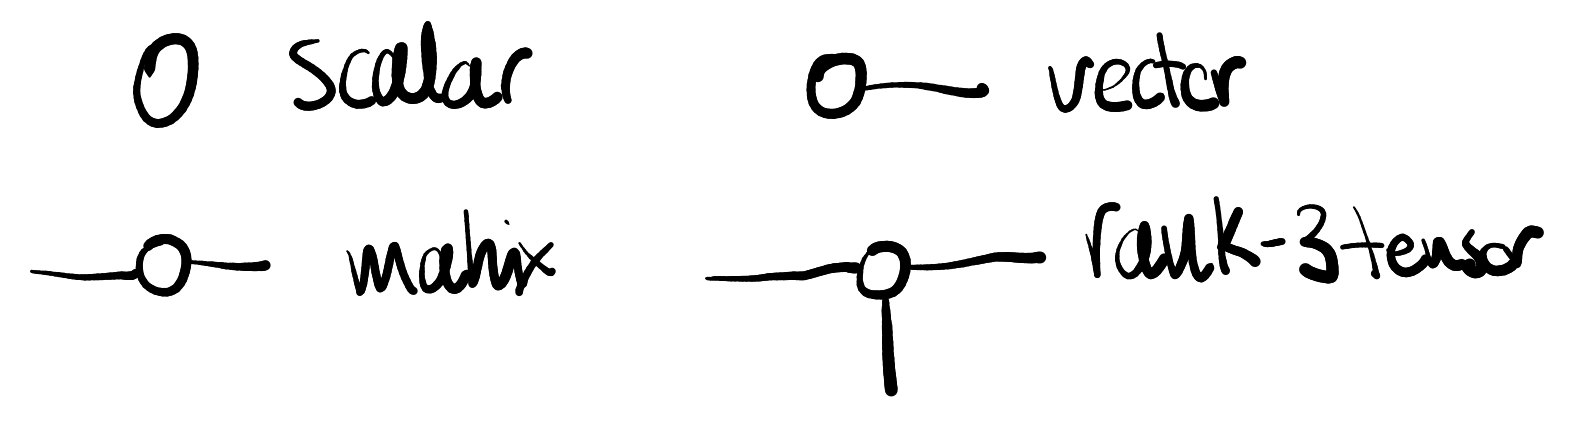
\includegraphics[scale=0.2]{graphs/TNpieces.png}
            \caption{Diagram representation of tensors. The tensors are the shapes and their indices are the lines emerging from.}
            \label{fig:TNpieces}
        \end{figure}

		Introduce a diagrammatic way to visual them, as in \autoref{fig:TNpieces}. A TN thus consists in interconnected such shapes. The lines between two different tensors corresponds to contracted indices, and those which do not connect two tensors are open indices. For instance, the trace of a product of $6$ matrices in represented in \autoref{fig:TNtrace}

		\begin{figure}[h!]
            \centering
            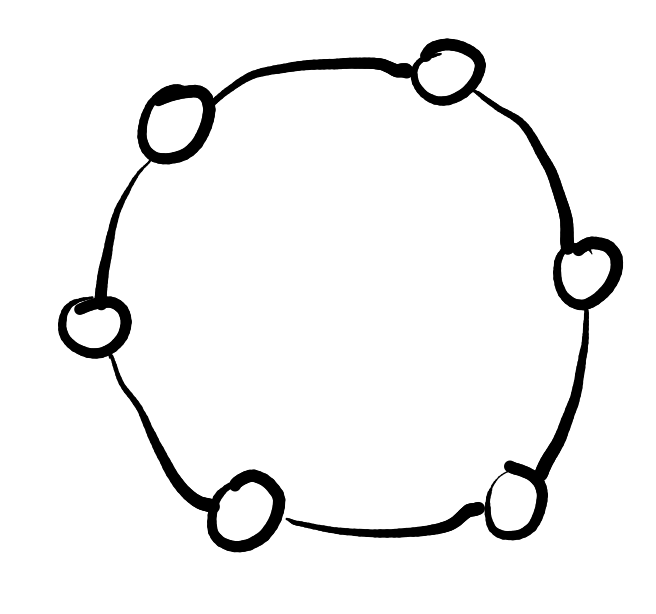
\includegraphics[scale=0.2]{graphs/TNtrace.png}
            \caption{Example of a trace of a product of $6$ matrices.}
            \label{fig:TNtrace}
        \end{figure}

    \section{Matrix product states}

    	For the Heisenberg antiferromagnet for example, the Hilbert space grows like $2^L$ with $L$ the number of sites. The ground state is hidden in a sea of non-relevant states for the problem. It lies in the corner of the Hilbert space one has already made allusion to, and can be found using methods that shall be presented later on. This corner can be represented by a matrix product state.

    	First recall the singular value decomposition. In the compact form, a $n\times m$ matrix $M$ can be decomposed as
    	\be M = U S V^\dagger \ee
    	with $U$ having orthonormal columns, $V^\dagger$ orthonormal rows and $S$ diagonal containing the singular values of $M$ order in descending way. The further goal is to approximate $M$ of rank $r$ --- that is the number of non-zero singular values --- by $M'$ of rank $r'<r$ by keeping only the largest singular values of $M$.

    	With sites $i=1,\dotsc, L$, write local $d$-dimensional states as $\{\sigma_i\}$. Take for now $d=1$, and write the most general pure state
    	\be \ket \psi = \sum_{\sigma_1,\dotsc,\sigma_L} c_{\sigma_1,\dotsc,\sigma_L} \ket{\sigma_1,\dotsc,\sigma_L} \ee
    	The goal is to find a notation that that enhances the locality of the states while preserving the non-locality of the state due to its quantum nature. Use SVD. One way of doing this is by left-canonical matrix product state. Reshape the states with $d^L$ components to one with $d\times d^{L-1}$, with coefficients
    	\be \Psi_{\sigma_1,(\sigma_2,\dotsc,\sigma_L)} = c_{\sigma_1,\dotsc,\sigma_L} \ee
    	Perform a SVD on $\Psi$
    	\be \begin{split} c_{\sigma_1,\dotsc,\sigma_L} &= \Psi_{\sigma_1,(\sigma_2,\dotsc,\sigma_L)} \\ &= \sum_{a_1=1}^{r_1} U_{\sigma_1,a_1} S_{a_1,a_1} (V^\dagger)_{a_1,(\sigma_2,\dotsc,\sigma_L)} \\ &= \sum_{a_1=1}^{r_1} U_{\sigma_1,a_1} c_{a_1\sigma_2,\dotsc,\sigma_L} \end{split} \ee
    	where $r_1\leq d$. Decompose $U$ in $d$ row vectors $A^{\sigma_1}$ as $A^{\sigma_1}_{a_1} = U_{\sigma_1,a_1}$. Reshape again $c_{a_1\sigma_2,\dotsc,\sigma_L} $ into a $r_1 d \times d^{L-2}$ matrix $\Psi_{(a_1\sigma_2),(\sigma_3,\dotsc,\sigma_L)}$ to get
    	\be c_{\sigma_1,\dotsc,\sigma_L} = \sum_{a_1=1}^{r_1} A^{\sigma_1}_{a_1} \Psi_{(a_1\sigma_2),(\sigma_3,\dotsc,\sigma_L)}\ee
    	Continue this procedure as
    	\be \begin{split} c_{\sigma_1,\dotsc,\sigma_L} &= \sum_{a_1=1}^{r_1} \sum_{a_2=1}^{r_2} A^{\sigma_1}_{a_1} U_{(a_1\sigma_2),a_2} S_{a_2,a_2} (V^\dagger)_{a_2,(\sigma_3,\dotsc,\sigma_L)} \\ &= \sum_{a_1=1}^{r_1} \sum_{a_2=1}^{r_2} A^{\sigma_1}_{a_1} A^{\sigma_2}_{a_1,a_2} \Psi_{(a_2\sigma_3),(\sigma_4,\dotsc,\sigma_L)} \end{split} \ee
    	with $A^{\sigma_2}_{a_1,a_2} =  U_{(a_1\sigma_2),a_2}$ and $A^{\sigma_2}$ a $r_1\times r_2$ matrix. Also, $\Psi_{(a_2\sigma_3),(\sigma_4,\dotsc,\sigma_L)}$ a $r_2d\times d^{L-3}$ matrix, with $r_2\leq r_1 d$. Continue to have
    	\be \begin{split} c_{\sigma_1,\dotsc,\sigma_L} &= \sum_{a_1,\dotsc,a_{L-1}} A^{\sigma_1}_{a_1} A^{\sigma_2}_{a_1,a_2} \cdots A^{\sigma_{L-1}}_{a_{L-2},a_{L-1}} A^{\sigma_L}_{a_{L-1}} \\ &= A^{\sigma_1} A^{\sigma_2} \cdots A^{\sigma_{L-1}} A^{\sigma_L} \end{split} \ee
    	Finally giving
    	\be \ket \psi = \sum_{\sigma_1,\dotsc,\sigma_L} A^{\sigma_1} A^{\sigma_2} \cdots A^{\sigma_{L-1}} A^{\sigma_L} \ket{\sigma_1,\dotsc,\sigma_L} \ee
    	However, considering $L$ even for simplicity, the maximum dimension of the $A$ matrices is $d^{L/2-1}\times d^{L/2}$ which makes the computation untenable.

    \section{AKLT as a MPS}

    	Recall the parent Hamiltonian of the model as in \autoref{fig:AKLTVBS}
    	\be \mc H = \sum_i \vb* S_i \cdot \vb* S_{i+1} + \frac 1 3 [ \vb* S_i \cdot \vb* S_{i+1}]^2 \ee
    	Taking $S=1$ symmetrized states at the sites as pairs of spins-$\frac 1 2$ and singlet linking them, one has for the $S=1$ states
    	\be \begin{split} \ket + &= \ket{\uparrow \uparrow} \\ \ket - &= \ket{\downarrow \downarrow} \\ \ket 0 &= \frac 1 2 [\ket{\uparrow \downarrow} + \ket{\downarrow \uparrow}] \end{split} \label{eq:TNAKLTS1} \ee
    	and for the valence bond singlets $\frac 1 2 [\ket{\uparrow \downarrow} - \ket{\downarrow \uparrow}]$. In the language of $2L$ spin-$\frac 1 2$ states, a state is
    	\be \ket \psi = \sum_{\vb* a,\vb* b} c_{\vb* a,\vb* b} \ket{\vb* a,\vb* b} \ee
    	Moreover, a state on site $i$ is
    	\be \ket{\Sigma^i} = \sum_{b_i,a_{i+1}} \Sigma_{ba} \ket{b_i} \ket{a_{i+1}} \ee
    	and introducing the matrix $\Sigma$ as
    	\be \Sigma = \pmqty{0 & \frac{1}{\sqrt 2} \\ - \frac{1}{\sqrt 2} & 0} \ee
    	Hence, write the state with singlets on all bonds
    	\be \ket{\psi_\Sigma} = \sum_{\vb* a,\vb* b} \Sigma_{b_1a_2} \Sigma_{b_2a_3} \cdots \Sigma_{b_La_1} \ket{\vb* a,\vb* b} \ee

    	\begin{figure}[h!]
            \centering
            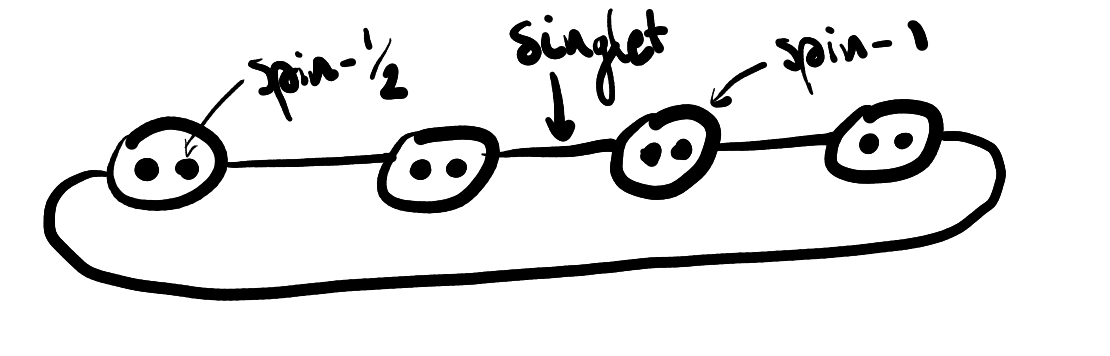
\includegraphics[scale=0.2]{graphs/AKLTVBS.png}
            \caption{Example of AKLT model for $S=1$ states with periodic BCs.}
            \label{fig:AKLTVBS}
        \end{figure}

        All is written is the spin-$\frac 1 2$ language, thus map $\ket{a_i}\ket{b_i} \in \{\ket \uparrow, \ket \downarrow \}^{\otimes2}$ to the physical spin-1 states $\ket{\sigma_i} \in \{\ket + , \ket 0, \ket - \}$. Thus to represent \eqref{eq:TNAKLTS1}, introduce matrices
        \be \begin{split} M^+ &= \pmqty{1 & 0 \\ 0 & 0} \\ M^0 &= \pmqty{0 & \frac{1}{\sqrt 2} \\ \frac{1}{\sqrt 2} & 0} \\ M^- &=  \pmqty{0 & 0 \\ 0 & 1} \end{split} \ee
        Then, one finds
        \be \ket{\sigma} = \sum_{a,b} M^\sigma_{ab} \ket{a,b} \ee
        Therefore, one has the mapping
        \be \begin{split} \ket{\psi_\Sigma} &\to \sum_{\vb* a,\vb* b, \vb* \sigma} M^{\sigma_1}_{a_1 b_1} \cdots M^{\sigma_L}_{a_L b_L} \ket{\vb* \sigma} \braket{\vb* \sigma}{\vb* a,\vb* b} \\ &= \sum_{\vb* a,\vb* b, \vb* \sigma} M^{\sigma_1}_{a_1 b_1} \Sigma_{b_1 a_2} \cdots M^{\sigma_L}_{a_L b_L} \Sigma_{b_L a_1} \ket{\vb* \sigma} \\ &= \sum_{\vb* \sigma} \tr [M^{\sigma_1} \Sigma M^{\sigma_2} \Sigma \cdots M^{\sigma_L} \Sigma ] \ket{\vb* \sigma} \\ &= \ket \psi \end{split} \ee
        Simply by further denoting $\widetilde A^\sigma = M^\sigma \Sigma$ with
        \be \begin{split} \widetilde A^+ &= \pmqty{0 & \frac{1}{\sqrt 2} \\ 0 & 0} \\ \widetilde A^0 &= \pmqty{-\frac{1}{2} & 0 \\ 0 & \frac{1}{2}} \\ \widetilde A^- &=  \pmqty{0 & 0 \\ -\frac{1}{\sqrt 2} & 0} \end{split} \ee
        giving
        \be \ket \psi = \sum_{\vb* \sigma} \tr [\widetilde A^{\sigma_1} \cdots \widetilde A^{\sigma_L}] \ket{\vb* \sigma} \ee
        which is not normalized. Thus left-normalize the $\widetilde A^\sigma$. Since
        \be \sum_\sigma \widetilde A^{\sigma^\dagger} \widetilde A^\sigma = \frac 3 4 \mathbb 1 \ee
        Hence rescale to obtain $A^\sigma$ matrices as
        \be \begin{split} A^+ &= \pmqty{0 & \sqrt{\frac 2 3} \\ 0 & 0} \\ A^0 &= \pmqty{-\frac{1}{\sqrt 3} & 0 \\ 0 & \frac{1}{\sqrt 3}} \\ A^- &=  \pmqty{0 & 0 \\ -\sqrt{\frac 2 3} & 0} \end{split} \ee
        This allows finally to compute
        \be \begin{split} \braket{\psi} &= \sum_{\vb* \sigma,\vb* \sigma'} \tr  [A^{\sigma'_1} \cdots A^{\sigma'_L}]^\dagger \tr [A^{\sigma_1} \cdots A^{\sigma_L}] \braket{\vb* \sigma'}{\vb* \sigma} \\ &\stackrel{[1]}{=} \sum_{\vb* \sigma} \tr [A^{\sigma_1} \cdots A^{\sigma_L}]^* \tr [A^{\sigma_1} \cdots A^{\sigma_L}] \\ &\stackrel{[2]}{=} \sum_{\vb* \sigma} \tr  [A^{\sigma^*_1} \cdots A^{\sigma^*_L}] \tr [A^{\sigma_1} \cdots A^{\sigma_L}] \\ &\stackrel{[3]}{=} \sum_{\vb* \sigma} \tr [(A^{\sigma^*_1} \cdots A^{\sigma^*_L}) \otimes (A^{\sigma_1} \cdots A^{\sigma_L})] \\ &\stackrel{[4]}{=} \tr \left[ \left( \sum_{\sigma_1} A^{\sigma^*_1} \otimes A^{\sigma_1}\right) \cdots \left( \sum_{\sigma_1} A^{\sigma^*_L} \otimes A^{\sigma_L}\right)\right] \\ &= \tr E^L \\ &= 1+ 3\left(-\frac 1 3 \right)^L \xrightarrow{L\to \infty} 1 \end{split} \ee
        where
        \be E = \sum_\sigma A^{\sigma^*} \otimes A^\sigma = \pmqty{\frac 1 3 & 0 & 0 & \frac 2 3 \\ 0 & -\frac 1 3 & 0 & 0 \\ 0 & 0 & -\frac 1 3 & 0 \\ \frac 2 3 & 0 & 0 & \frac 1 3} \ee
        that has eigenvalues $1,-\frac 1 3,-\frac 1 3,-\frac 1 3$. The relations used are the following
        \begin{enumerate}[label=${[\arabic*]}\rightarrow$]
        	\item $\tr A^\dagger = \tr A$
        	\item $\tr (A)^* = \tr A^*$
        	\item $\tr A\otimes B = \tr A \tr B$
        	\item $(AB)\otimes(CD) = (A\otimes C)(B\otimes D)$
    	\end{enumerate}

    	Hence, it has been possible to express the AKLT model as a $d=2$ matrix product state.

    \section{Entanglement entropy}

        Here, one derives the Schmidt decomposition of a general quantum state. First, a pure state is written 
        \be \ket \psi = \sum_{ij} \Psi_{ij} \ket i_A \ket j_B \ee
        on $\mc H_A \otimes \mc H_B$, with basis $\dim \{\ket i_A\}=N_A$ and $\dim \{\ket j_B\}=N_B$, which has density operator $\hat \rho = \dyad{\psi}$. The reduced density operators are thus the partial traces
        \be \hat \rho_A = \tr _B \dyad{\psi} \qq{and} \hat \rho_B = \tr _A \dyad{\psi} \ee
        Perform SVD on matrix $\Psi$, then
        \be \begin{split} \ket \psi &= \sum_{ij} \sum_{a=0}^{\min(N_1,N_B)} U_{ia}S_{aa}V^*_{ja} \ket i_A \ket j_B \\ &= \sum_{a=0}^{\min(N_1,N_B)} \left(\sum_i U_{ia} \ket i_A \right) s_a \left(\sum_j V^*_{ja} \ket j_B\right) \\ &=  \sum_{a=0}^{\min(N_1,N_B)} s_a \ket a_A \ket a_B \end{split} \ee
        Truncate to the $r\leq \min(N_1,N_B)$ largest singular values to get
        \be \ket \psi = \sum_{a=1}^r s_a \ket a_A \ket a_B \ee
        and this is the Schmidt decomposition. For $r>1$ the system is entangled. The reduced density operators then read
        \be \hat \rho_A = \sum_{a=1}^r s_a^2 \dyad{a_A} \qq{and} \hat \rho_B = \sum_{a=1}^r s_a^2 \dyad{a_B} \ee 
        The eigenvalues being $s_a^2$ and the eigenvectors left- and right-singular vectors, allow to write the von Neumann entropy of entanglement defined as $S(\rho) = - \tr \rho \ln \rho$, as
        \be S_A(\ket \psi) = -\tr \hat \rho_A \ln \hat \rho_A = - \sum_{a=1}^r s_a^2 \ln s_a^2 \ee
        and note that $S_B(\ket \psi) = S_A(\ket \psi)$.

    \section{Correlation length for AKLT}

        To calculate observables, one defines the operators that act as
        \be \hat O^{[l]} = \sum_{\sigma_l,\sigma'_l} O^{\sigma_l,\sigma'_l} \dyad{\sigma_l}{\sigma'_l} \ee
        The goal her is to calculate the correlations on a translationally invariant state with left-normalized site-independent $A$ matrices and thus $E$ matrices=. Then
        \be \begin{split} &\quad \ev{\hat O^{[i]} \hat O^{[j]}}{\psi} \\ &= \tr\left[E^{[1]}\cdots E^{[i-1]}E_O^{[i]}E^{[i+1]} \cdots E^{[j-1]}E_O^{[j]}E^{[j+1]} \cdots E^{[L]}\right] \\ &= \tr\left[E_O^{[i]} E^{j-i-1} E_O^{[j]}E^{L-j+i-1} \right] \\ &= \sum_{k,l} \mel{l}{E_O^{[i]}}{k} \lambda^{j-i-1}_k \mel{k}{E_O^{[j]}}{l} \lambda_l^{L-j+i-1} \\ &\xrightarrow{L\to \infty} \sum_k \mel{1}{E_O^{[i]}}{k} \lambda^{j-i-1}_k \mel{k}{E_O^{[j]}}{1} \end{split} \ee
        with $E_O$ having the interposed operator $\hat O$ and since $\lambda_1=1$ and $\abs{\lambda_k} < 1 \ \forall k>1$. Hence, if $\mel{1}{E_O^{[i]}}{1}$ are finite, the correlations can be long-ranged, else they are a superposition of exponentials with decay length $\xi_k = - \frac{1}{\ln \lambda_k}$, thus 
        \be \frac{\ev{\hat O^{[i]} \hat O^{[j]}}{\psi}}{\braket{\psi}} = c_1 + \sum_{k=2}^{D^2} c_k e^{\frac{r}{\xi_k}} \ee
        with $r=\abs{j-i-1}$ and $c_k = \mel{1}{E_O^{[i]}}{k}\mel{k}{E_O^{[j]}}{1}$. For AKLT and $i<j$,
        \be \ev{S_i^z S_j^z} = \frac{12}{9} (-1)^{j-i} e^{-(j-i)\ln 3} \ee
        hence $\xi = \frac{1}{\ln 3}$.

    \section{Bring a MPS to canonical form}
    
        Start with a general MPS without normalization
        \be \begin{split} \ket \psi &= \sum_{\sigma_1,\dotsc,\sigma_L} M^{\sigma_1} M^{\sigma_2} \cdots M^{\sigma_{L-1}} M^{\sigma_L} \ket{\sigma_1,\dotsc,\sigma_L} \\ &= \sum_{\vb* \sigma} \sum_{a_1,\dotsc,a_{L-1}} M^{\sigma_1}_{1,a_1} M^{\sigma_2}_{a_1,a_2} \cdots M^{\sigma_{L-1}}_{a_{L-2},a_{L-1}} M^{\sigma_L}_{a_{L-1},1} \ket{\vb* \sigma} \\ &= \sum_{\vb* \sigma} \sum_{a_1,\dotsc,a_{L-1}} M_{(\sigma_1,1),a_1} M^{\sigma_2}_{a_1,a_2} \cdots M^{\sigma_{L-1}}_{a_{L-2},a_{L-1}} M^{\sigma_L}_{a_{L-1},1} \ket{\vb* \sigma} \\ &\stackrel{\text{SVD}}{=} \sum_{\vb* \sigma} \sum_{a_1,\dotsc,a_{L-1}} \sum_{s_1} A_{(\sigma_1,1),s_1} S_{s_1,s_1} V^\dagger_{s_1,a_1} M^{\sigma_2}_{a_1,a_2} \cdots \ket{\vb* \sigma} \\ &= \sum_{\vb* \sigma} \sum_{a_2,\dotsc,a_{L-1}} \sum_{s_1} A^{\sigma_1}_{1,s_1} \underbrace{\left[\sum_{a_1} S_{s_1,s_1} V^\dagger_{s_1,a_1} M^{\sigma_2}_{a_1,a_2} \right]}_{\widetilde M^{\sigma_2}_{s_1,a_2}} M^{\sigma_3}_{a_2,a_3} \cdots \ket{\vb* \sigma} \end{split} \ee
        and $A^\dagger A= \mathbb 1$ due to SVD is left-normalization. Iterate the procedure to get MPS with $\widetilde M$s. To do so, reshape $\widetilde M^{\sigma_2}_{s_1,a_2}$ to $\widetilde M^{(\sigma_2,s_1),a_2}$, do SVD to get $A_{(\sigma_2,s_1),a_2}$ which is reshape to a left-normalized $A^{\sigma_2}_{s_1,s_2}$. Multiply the two right matrices of this SVD with the left $M$ matrix to repeat the process. In the end, has left-normalized $A^{\sigma_i}_{s_{i-1},s_i}$ on all site except the last one having a remaining scalar $S_{1,1}V^\dagger_{1,1}$ which corresponds to the norm of $\ket \psi$.

    \section{Matrix product operator}
        
        \begin{figure}[h!]
            \centering
            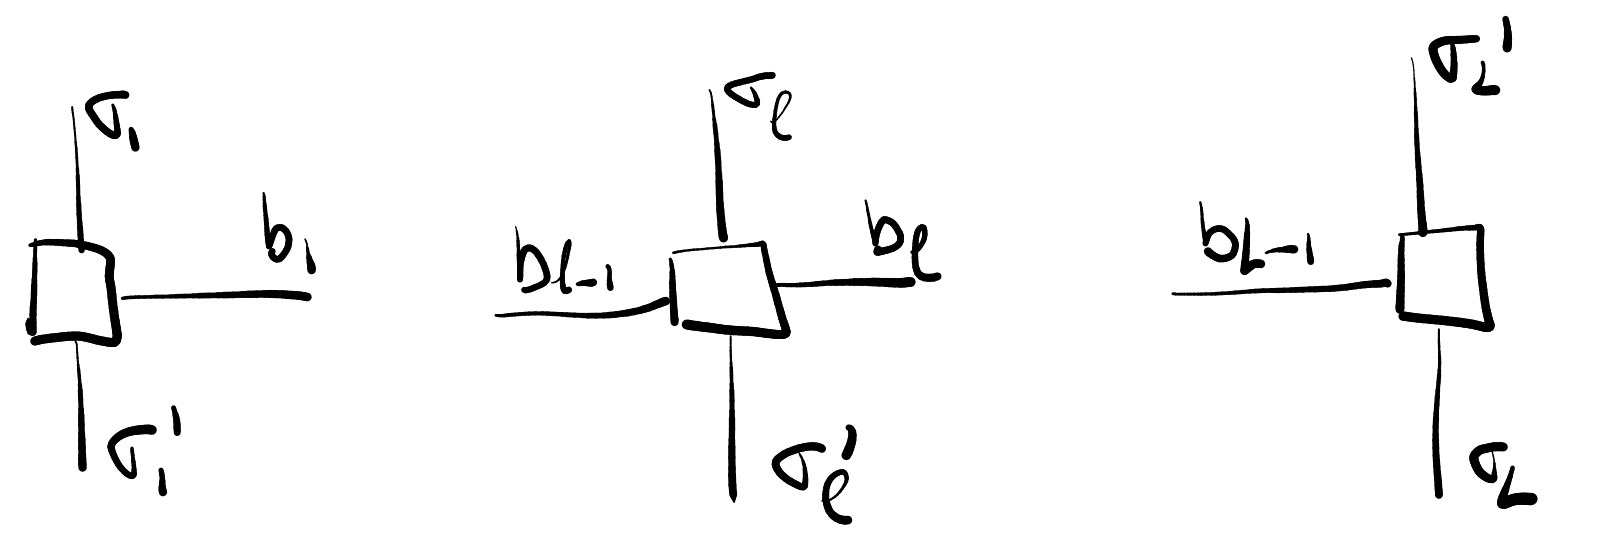
\includegraphics[scale=0.2]{graphs/physmpotn.png}
            \caption{Elements of a matrix product operator with physical indices pointing up and down.}
            \label{fig:physmpotn}
        \end{figure}

        An operator $\hat O: H \to H$ with $\{\ket{A_i}\}$ an orthonormal basis of $H$ can be written as
        \be \begin{split} \hat O &= \sum_i \dyad{A_i} \hat O \sum_j \dyad{A_j} \\ &= \sum_{ij} O_{ij} \dyad{A_i}{A_j} \end{split} \ee
        and writing $H = \otimes_{i=1}^L H_s$ one gets
        \be \hat O = \sum_{\vb* \sigma,\vb* \sigma'} O_{(\sigma_1,\dotsc,\sigma_L),(\sigma_1',\dotsc,\sigma_L')} \dyad{\sigma_1,\dotsc,\sigma_L}{\sigma_1',\dotsc,\sigma_L'} \ee
        the general form of an operator in tensorial state. Reshaping
        \be O_{(\sigma_1,\dotsc,\sigma_L),(\sigma_1',\dotsc,\sigma_L')} = c_{(\sigma_1,\sigma_1'),\dotsc,(\sigma_L,\sigma_L')} \ee
        enables to decompose in canonical form as for the MPS to get a MPO
        \be \hat O = \sum_{\vb* \sigma,\vb* \sigma'} W^{\sigma_1,\sigma_1'} \cdots W^{\sigma_L,\sigma_L'} \dyad{\vb* \sigma}{\vb* \sigma'} \ee
        Now, instead of having one physical state, there are two, shown on \autoref{fig:physmpotn}, and thus the MPO looks as in \autoref{fig:mpotnrep}.
        
        \begin{figure}[h!]
            \centering
            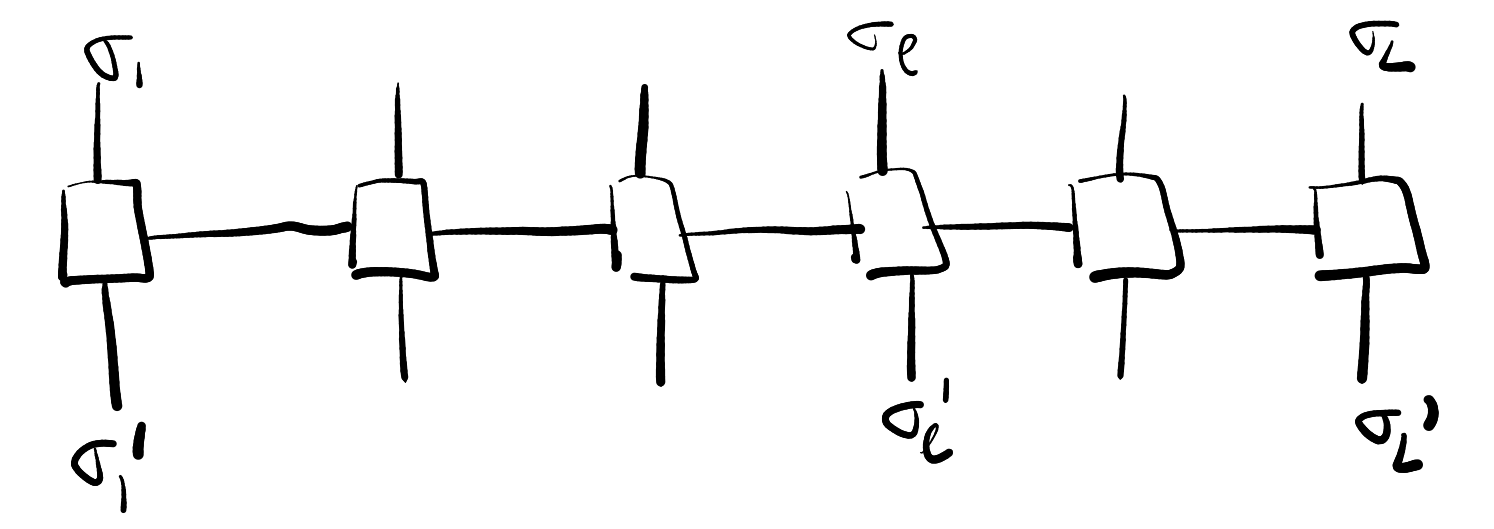
\includegraphics[scale=0.2]{graphs/mpotnrep.png}
            \caption{A MPO acting on a chain, ready to be applied to a MPS.}
            \label{fig:mpotnrep}
        \end{figure}

        Now apply the MPO to a MPS 
        \be \begin{split} \hat O \ket \psi &= \sum_{\vb* \sigma,\vb* \sigma'} W^{\sigma_1,\sigma_1'} \cdots W^{\sigma_L,\sigma_L'} \ket{\vb* \sigma}\braket{\vb* \sigma'}{\psi} \\ &= \sum_{\vb* \sigma,\vb* \sigma'} W^{\sigma_1,\sigma_1'} \cdots W^{\sigma_L,\sigma_L'} M^{\sigma_1'} \cdots M^{\sigma_L'} \ket{\vb* \sigma} \\ &= \sum_{\vb* \sigma,\vb* \sigma'} \sum_{\vb* a,\vb* b} \left( W^{\sigma_1,\sigma_1'}_{1,b_1} W^{\sigma_2,\sigma_2'}_{b_1,b_2} \cdots\right) \left( M^{\sigma_1'}_{1,a_1} M^{\sigma_2'}_{a_1,a_2} \cdots\right) \ket{\vb* \sigma} \\ &= \sum_{\vb* \sigma,\vb* \sigma'} \sum_{\vb* a,\vb* b} \left( W^{\sigma_1,\sigma_1'}_{1,b_1} M^{\sigma_1'}_{1,a_1} \right) \left( W^{\sigma_2,\sigma_2'}_{b_1,b_2} M^{\sigma_1'}_{1,a_1} \right) \cdots \ket{\vb* \sigma} \\ &= \sum_{\vb* \sigma} \sum_{\vb* a,\vb* b} N^{\sigma_1}_{(1,1),(b_1,a_1)} N^{\sigma_2}_{(b_1,a_1),(b_2,a_2)} \cdots \ket{\vb* \sigma} \\ &= \sum_{\vb* \sigma} N^{\sigma_1} N^{\sigma_2} \cdots \ket{\vb* \sigma} \end{split} \ee
        which is still a MPS !

        \begin{figure}[h!]
            \centering
            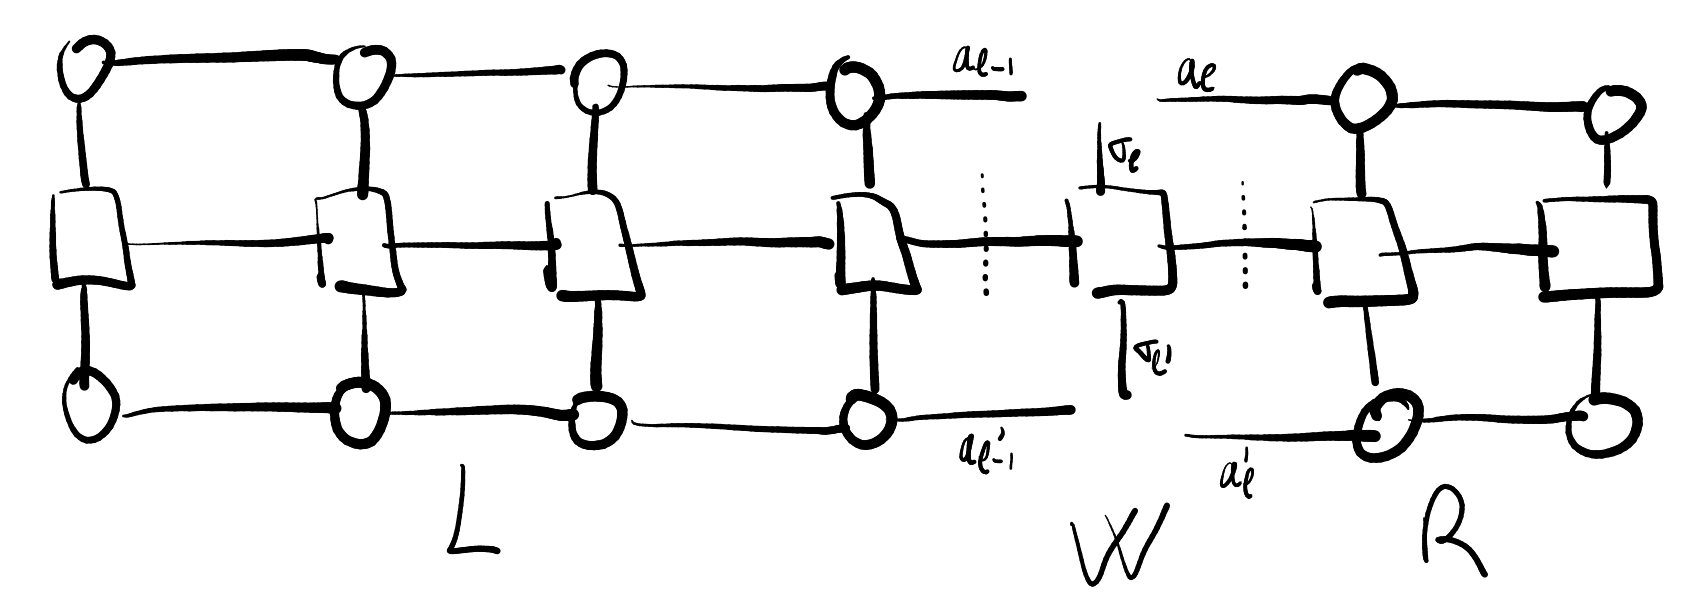
\includegraphics[scale=0.2]{graphs/mpohamdmrgtn.png}
            \caption{Representation of the DRMG Hamiltonian matrix element in MPS/MPO language.}
            \label{fig:mpohamdmrgtn}
        \end{figure}

        To apply a Hamiltonian MPO on a mixed canonical state, consider the MPS 
        \be \begin{split} \ket \psi &= \sum_{\vb* \sigma} A^{\sigma_1} \cdots ^{\sigma_{\ell-1}} \Psi^{\sigma_\ell} B^{\sigma_{\ell+1}}\cdots B^{\sigma_L} \ket{\vb* \sigma} \\ &= \sum_{a_{\ell-1},a_\ell} \ket{a_{\ell-1}}_A \Psi^{\sigma_\ell}_{a_{\ell-1},a_\ell} \ket{a_\ell}_B \end{split} \ee
        Then apply the Hamiltonian
        \be \begin{split} \mc H \ket \psi &= \sum_{a_{\ell-1},a_\ell} \Psi^{\sigma_\ell}_{a_{\ell-1},a_\ell} \mc H \ket{a_{\ell-1},\sigma_\ell,a_\ell} \\ &= \sum_{a_{\ell-1},a_\ell} \sum_{a_{\ell-1}',\sigma_\ell',a_\ell'} \Psi^{\sigma_\ell}_{a_{\ell-1},a_\ell} \mel{a_{\ell-1}',\sigma_\ell',a_\ell'}{\mc H}{a_{\ell-1},\sigma_\ell,a_\ell} \ket{a_{\ell-1}',\sigma_\ell',a_\ell'} \end{split} \ee
        where one writes, as in \autoref{fig:mpohamdmrgtn},
        \be \mel{a_{\ell-1}',\sigma_\ell',a_\ell'}{\mc H}{a_{\ell-1},\sigma_\ell,a_\ell} = \sum_{b_{\ell-1},b_\ell} L^{a'_{\ell-1},a_{\ell-1}}_{b_{\ell-1}} W^{\sigma'_\ell,\sigma_\ell}_{b_{\ell-1},b_\ell} R^{a'_{\ell},a_{\ell}}_{b_{\ell}} \ee

    \section{DMRG}
        
        Consider spin-$\frac 1 2$ nearest-neighbors Heisenberg antiferromagnetic chain of length $L$ with open BCs. DMRG prefers open BCs, and is for $L$ finite. iDMRG is for $L\to \infty$. The goal is to find the ground state energy of a Hamiltonian $\mc H$. It is adequate to run a two steps algorithm that starts with iDMRG to go to DMRG. Note that here the dimension of the Hilbert space is $d^L$, with $d=2$.
        
        \begin{figure}[h!]
            \centering
            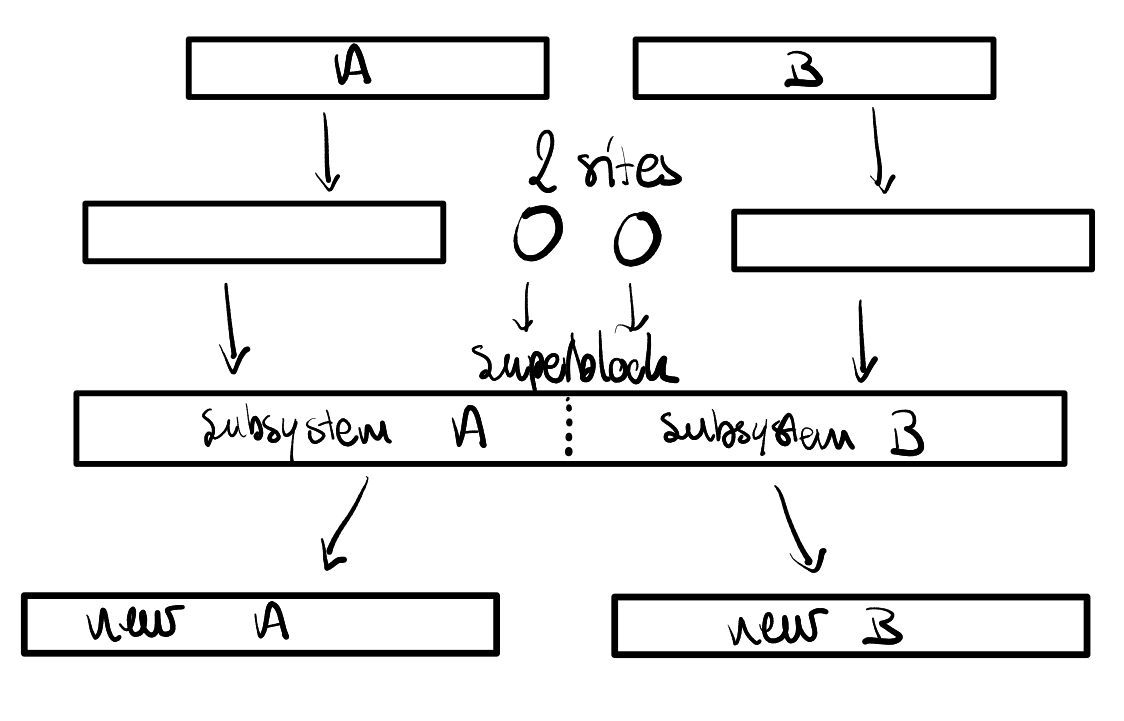
\includegraphics[scale=0.2]{graphs/idmrgsumup.png}
            \caption{iDMRG algorithm represented.}
            \label{fig:idmrgsumup}
        \end{figure}

        The iDMRG is proceeded as follows. The assumption is that there exists a reduced state that can describe the relevant physics and there exists a procedure to find it. Basically, consider a chain of increasing length an discard number of states to keep the algorithm efficient with manageable Hilbert space size. This is the decimation procedure. The iDMRG is sum up in \autoref{fig:idmrgsumup}. Introduce left and right blocks $A$ and $B$, which in a first step may consist of one spin each, such that total chain length is $2$. Longer chains are now built iteratively from the left and right end, by inserting pairs of spins between the blocks, such that the chain grows to length $4$, $6$, and so on. At each step, previous spins are absorbed into the left and right blocks, such that block sizes grow as $1$, $2$, $3$, and so on, leading to exponential growth of the dimension of the full block state space as $2^\ell$, where $\ell$ is the current block size. The chains then always have a block-site-site-block structure, $A\bullet \bullet \ B$. To find the ground state, say that any state in the superblock is
        \be \begin{split} \ket \psi &= \sum_{a_A=1}^D \sum_{\sigma_A=1}^d \sum_{\sigma_B=1}^d \sum_{a_B=1}^D \Psi_{a_A,\sigma_A,\sigma_B,a_B} \ket{a}_A \ket{\sigma}_A \ket{\sigma}_B\ket{a}_B \\ &= \sum_{i_Aj_B} \Psi_{i_A,j_B} \ket{i}_A \ket{j}_B \end{split} \ee
        where $D$ is chosen to be the dimension of the reduced Hilbert space of each block, and $\{\ket{a}_A\}$ forming a $D$-dimensional basis of the block $A$ for instance. Then minimize the energy 
        \be E = \frac{\ev{\mc H_{A\bullet \bullet \ B}}{\psi}}{\braket{\psi}} \ee
        with respect to the Hamiltonian of the superblock, to find the coefficients $\psi_{a_A,\sigma_A,\sigma_B,a_B}$ to have a good approximation of the ground state energy. If now the states $\{\ket{i}_A\}$ as the basis of the blocks $A\bullet$, the dimension of this basis is then $Dd$. To avoid exponential growth, truncate the basis back to $D$. To motivate, one wants to find the state $\ket{\tilde \psi}$ such that $\braket{\psi}{\tilde \psi}$ is minimized.

        The finite-size DMRG is shown on \autoref{fig:dmrgalgosumup}. It continues the growth process of \emph{eg} block $B$ following the same prescription as before. But it does so at the expense of block $A$, which shrinks \emph{ie} old shorter blocks $A$ are reused. This is continued until $A$ is so small as to have a complete Hilbert space. Then the growth direction is reversed. $A$ grows at the expense of $B$, including new ground state determinations and basis choices for $A$, until $B$ is small enough to have a complete Hilbert space, which leads to yet another reversal of growth direction. This sweeping through the system is continued until energy converges. The intuitive motivation for this procedure is that after each sweep, blocks $A$ or $B$ are determined in the presence of an ever improved embedding.

        \begin{figure}[h!]
            \centering
            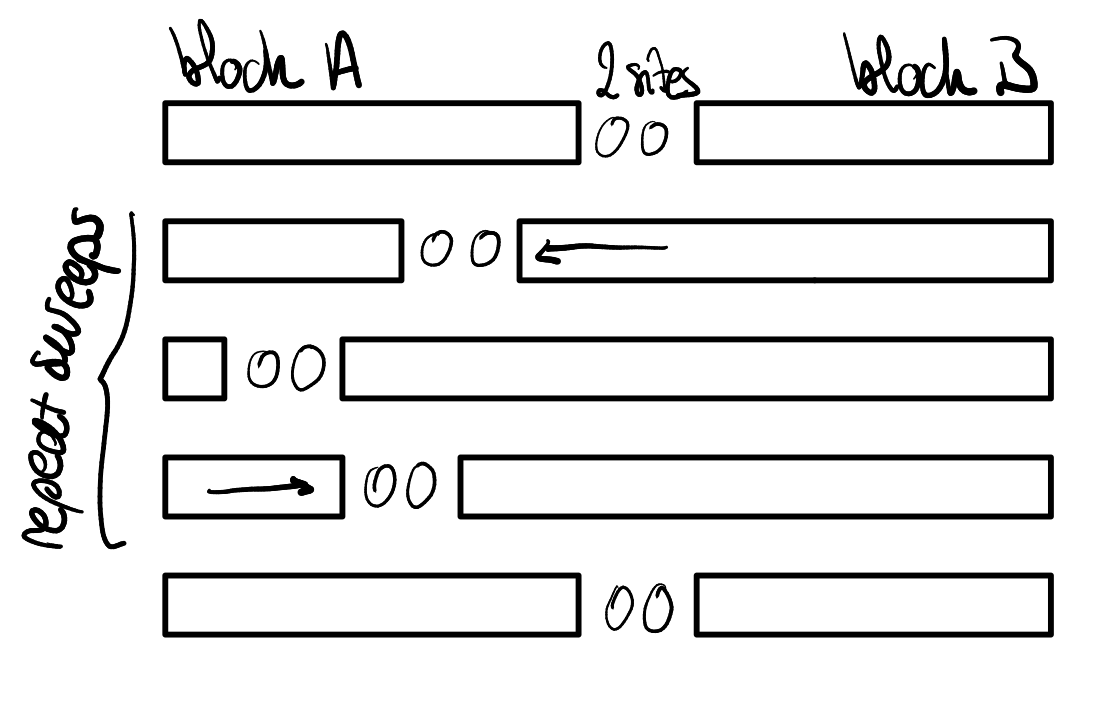
\includegraphics[scale=0.2]{graphs/dmrgalgosumup.png}
            \caption{DMRG algorithm summed up.}
            \label{fig:dmrgalgosumup}
        \end{figure}

        The ground state can be found using an iterative method by minimizing the energy $E = \frac{\ev{\mc H}{\psi}}{\braket{\psi}}$ thus finding
        \be \min_{\ket \psi, \lambda} \ev{\mc H}{\psi} - \lambda\braket{\psi} \ee
        The problem is that if one considers all the matrices $M$, the problem is highly non-linear. But one can proceed by keeping all the matrices on the sites except the one considered fixed. Of course, this is computationally worth --- quadratic form --- but not optimal. To calculate the terms of the minimization, note that it can be recast into a generalized eigenvalue problem
        \be \hat{\mc H}v - \lambda \hat{\mc N} v =0 \ee
        with $v_{\sigma_\ell,a_{\ell-1},a_\ell} = M^{\sigma_\ell}_{a_{\ell-1},a_\ell}$, which is represented in \autoref{fig:geneigdmrg}. If $\ket\psi$ is mixed canonical, thus left-normalized at the left of the site $\ell$ and right-normalized on the right, then $\mc N = \mathbb 1$, so that the problem reduces to \autoref{fig:geneigreduceddmrg}.

        \begin{figure}[h!]
            \centering
            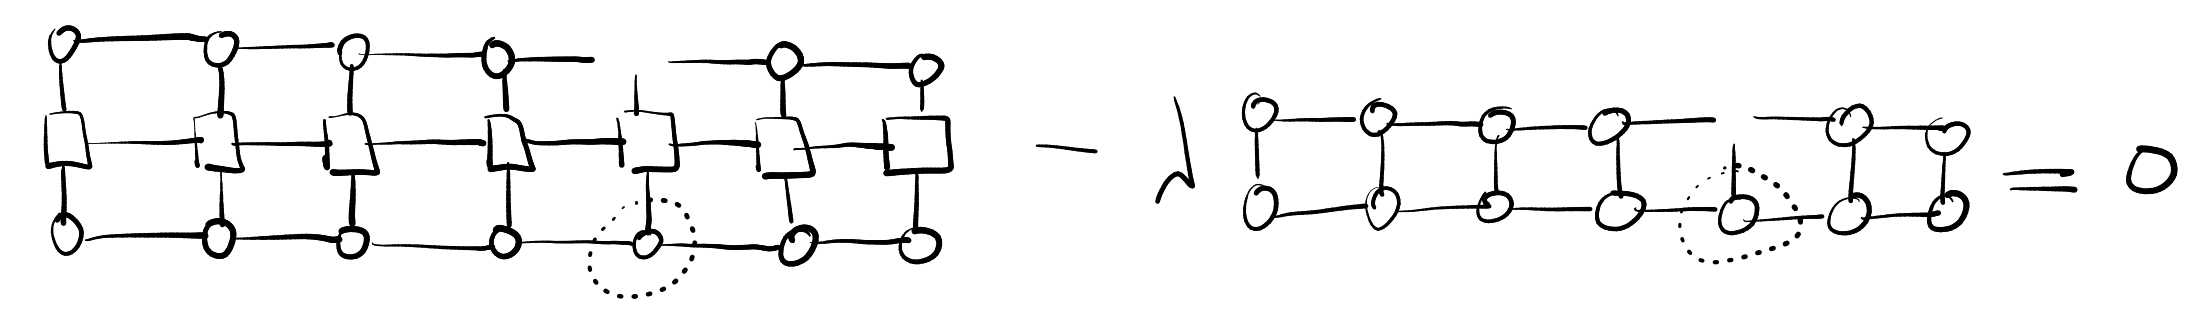
\includegraphics[width=\linewidth]{graphs/geneigdmrg.png}
            \caption{Generalized eigenvalue problem for the optimization of $v$.}
            \label{fig:geneigdmrg}
        \end{figure}

        The algorithm is as follows
        \begin{itemize}
            \item start for a random $\ket \psi$ 
            \item right-normalize it
            \item run the optimization from $\ell=1$ to $L-1$, that is, solve the eigenvalue problem for $M^{\sigma_\ell}$, then left-normalize it to $A^{\sigma_\ell}$ by SVD, absorb the $SV^\dagger$ into the $M^{\sigma_{\ell+1}}$, then move to the $\ell+1$ site and repeat until $L-1$
            \item start from $\ell = L$ to 2, and do the same but right-normalizing
            \item repeat the sweeps until convergence, but can fall in local minimum thus seek for the null error on the energy
        \end{itemize}

        \be \begin{split} &M_0 B_0 B_0 B_0 \cdots B_0 \\ \xrightarrow{\text{optimize}} &M_1 B_0 B_0 B_0 \cdots B_0 \xrightarrow{\text{SVD}} A_1 M_0 B_0 B_0 \cdots B_0 \\ \xrightarrow{\text{optimize}} &A_1 M_1 B_0 B_0 \cdots B_0 \xrightarrow{\text{SVD}} A_1 A_1 M_0 B_0 \cdots B_0 \\ \xrightarrow{\text{optimize}} &A_1 A_1 M_1 B_0 \cdots B_0 \xrightarrow{\text{SVD}} A_1 A_1 A_1 M_0 \cdots B_0 \\ \xrightarrow{\cdots} &A_1 A_1 A_1 A_1 \cdots M_0 \\ \xrightarrow{\text{optimize}}  &A_1 A_1 A_1 A_1 \cdots M_1 \xrightarrow{\text{SVD}} A_1 A_1 A_1 A_1 \cdots B_1 \\ \xrightarrow{\cdots} &A_1 A_1 A_1 M_1 \cdots B_1 \\ \xrightarrow{\text{optimize}} &A_1 A_1 A_1 M_2 \cdots B_1 \xrightarrow{\text{SVD}} A_1 A_1 M_1 B_2 \cdots B_1 \\ \xrightarrow{\text{optimize}} &A_1 A_1 M_2 B_2 \cdots B_1 \xrightarrow{\text{SVD}} A_1 M_1 B_2 B_2 \cdots B_1 \\ \xrightarrow{\text{optimize}} &A_1 M_2 B_2 B_2 \cdots B_1 \xrightarrow{\text{SVD}} M_1 B_2 B_2 B_2 \cdots B_1 \\ \xrightarrow{\cdots} & \end{split} \ee

        \begin{figure}[h!]
            \centering
            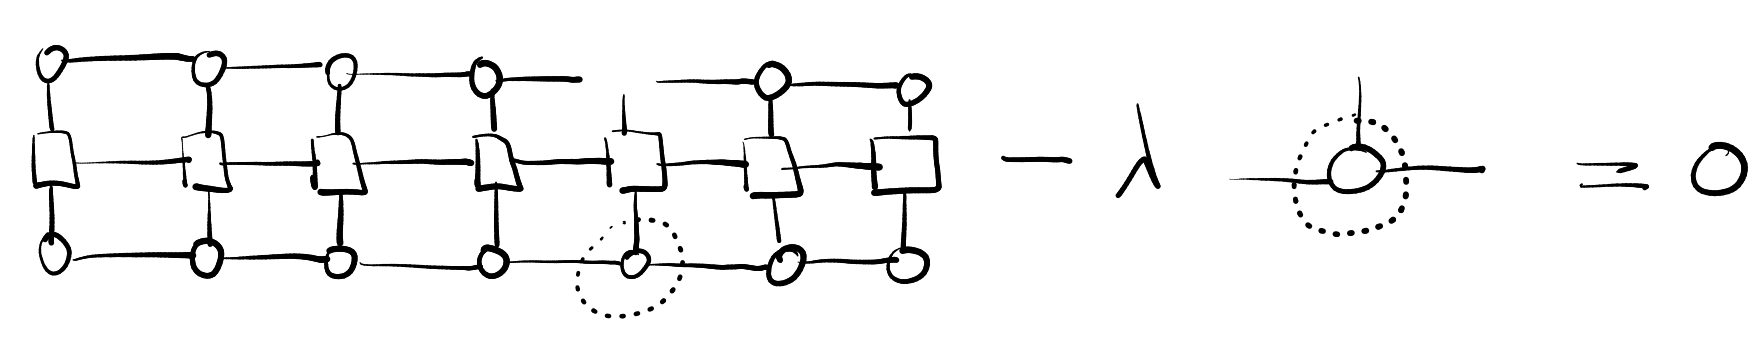
\includegraphics[width=\linewidth]{graphs/geneigreduceddmrg.png}
            \caption{Standard eigenvalue problem for the optimization of $v$.}
            \label{fig:geneigreduceddmrg}
        \end{figure}

    \section{Contractions of PEPS}
        
        Projected entangled pair states have an number of properties. They are translationally invariant, dense in the Hilbert space and increasing $D$ the bond dimension makes the corner increase in size, satisfy the area law of entanglement entropy. But they can have infinite correlation length, thus have no canonical form, and computing expectation values on them is exponentially costly. Hence, the order of contractions matters.
        
        \begin{figure}[h!]
            \centering
            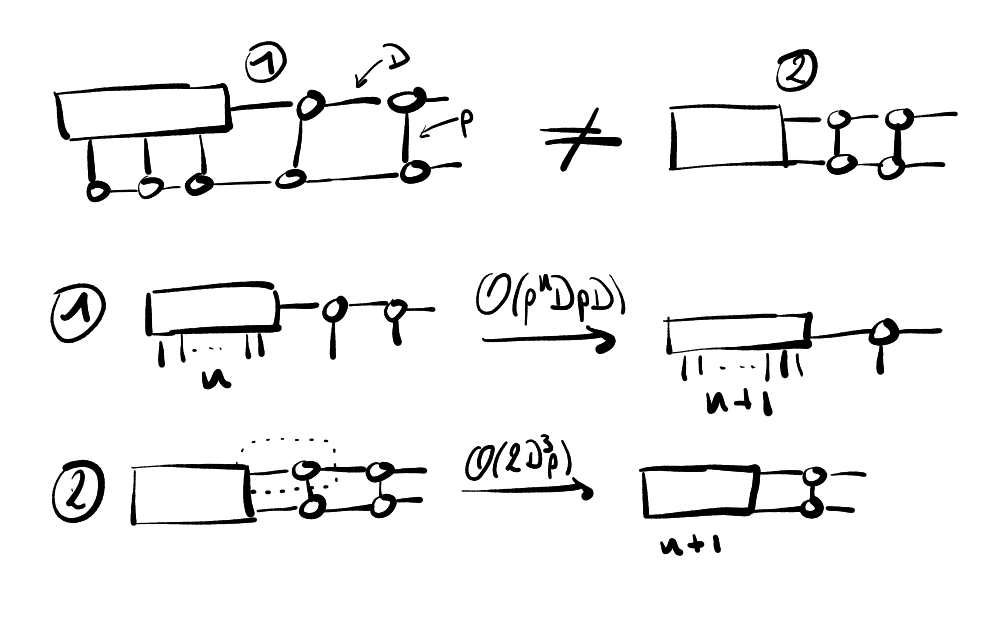
\includegraphics[scale=0.2]{graphs/pepsorder.png}
            \caption{Oder of contractions matters for the PEPS.}
            \label{fig:pepsorder}
        \end{figure}

        To see the difference in the order of contractions, look at \autoref{fig:pepsorder}. This is based on the property of contractions cost that is shown in \autoref{fig:contractionproptn}.

        \begin{figure}[h!]
            \centering
            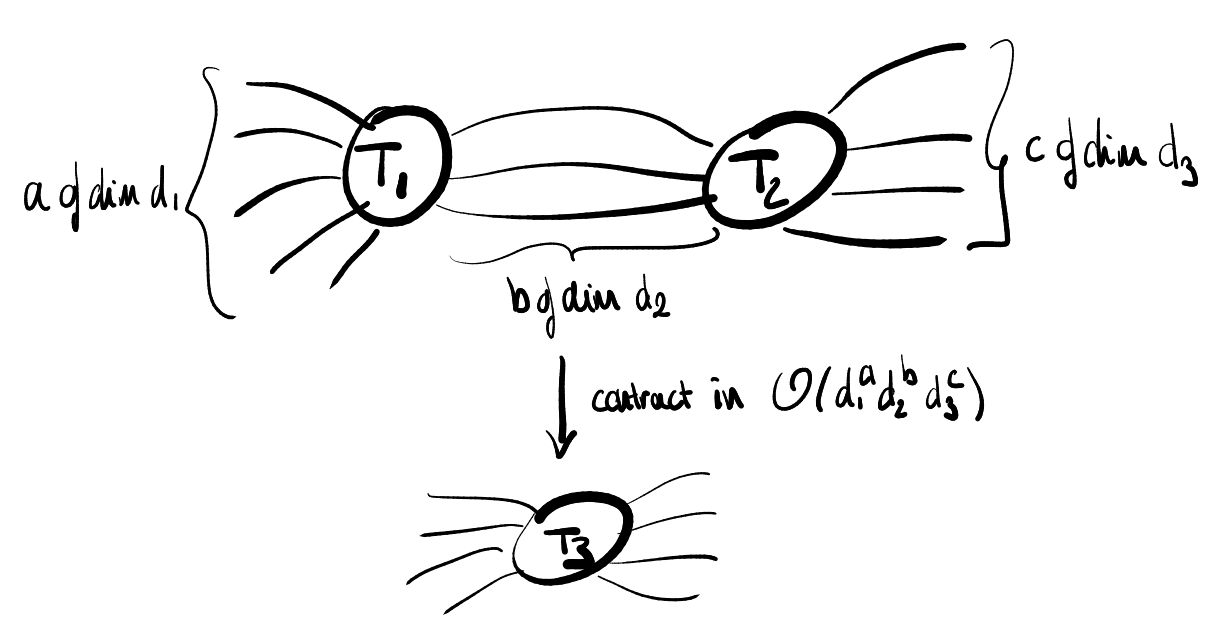
\includegraphics[scale=0.2]{graphs/contractionproptn.png}
            \caption{Property of the contractions cost for tensor networks.}
            \label{fig:contractionproptn}
        \end{figure}

        For a PEPS with bond dimension $D$, the contraction shown on \autoref{fig:pepscontractionD} is increasing exponentially in the linear number of sites, and this is anyway unavoidable.

        \begin{figure}[h!]
            \centering
            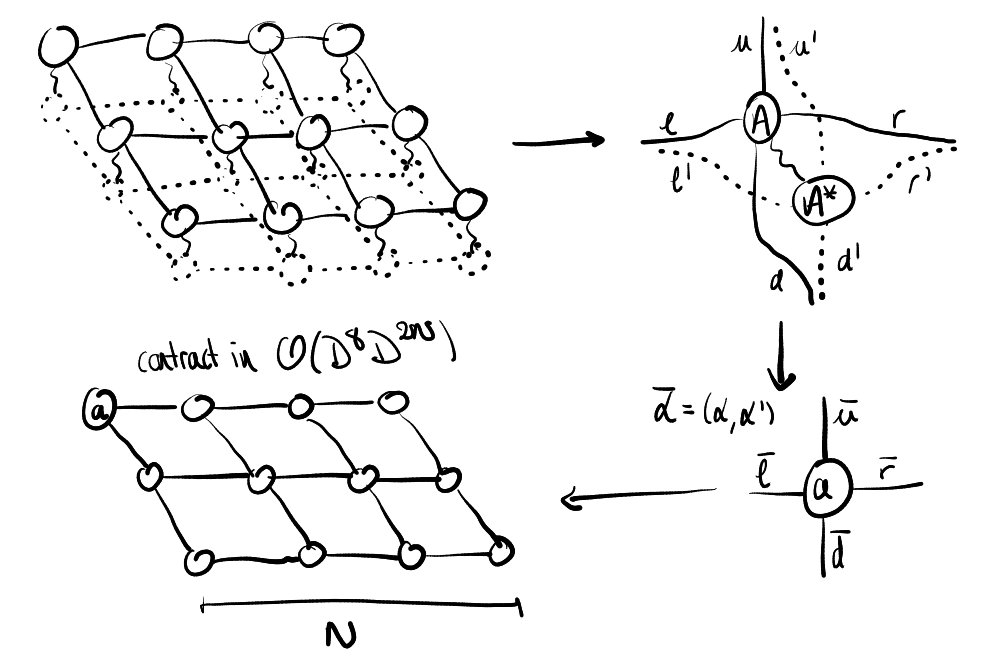
\includegraphics[scale=0.2]{graphs/pepscontractionD.png}
            \caption{Exponential cost of the PEPS contraction.}
            \label{fig:pepscontractionD}
        \end{figure}

    \section{CTMRG}
        
        There are basically two methods to find the ground state of a Hamiltonian, via imaginary time evolution of using a variational approach. In either case, the computations must be approximated, and this is where the corner transfer matrix renormalization group comes. This involves the computation of the environment of the system considered, and it becomes mandatory in the case of the infinite PEPS.

        \begin{figure}[h!]
            \centering
            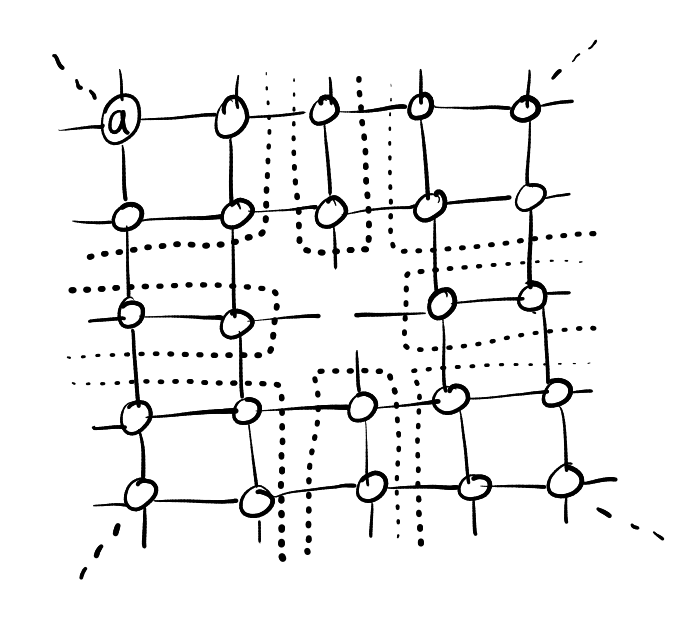
\includegraphics[scale=0.2]{graphs/envpepsctmrg.png}
            \caption{Environment of a tensor in the context of CTMRG.}
            \label{fig:envpepsctmrg}
        \end{figure}

        For a square lattice as used before, the environment is presented on \autoref{fig:envpepsctmrg}. Then, the goal is to compute an effective environment since the exact computation is to costly. The algorithm is therefore on \autoref{fig:ctmrgalgo}. Only one step is shown, $3$ others must be performed on each side --- or $\bar \alpha$ bond --- to complete one iteration.

        \begin{figure}[h!]
            \centering
            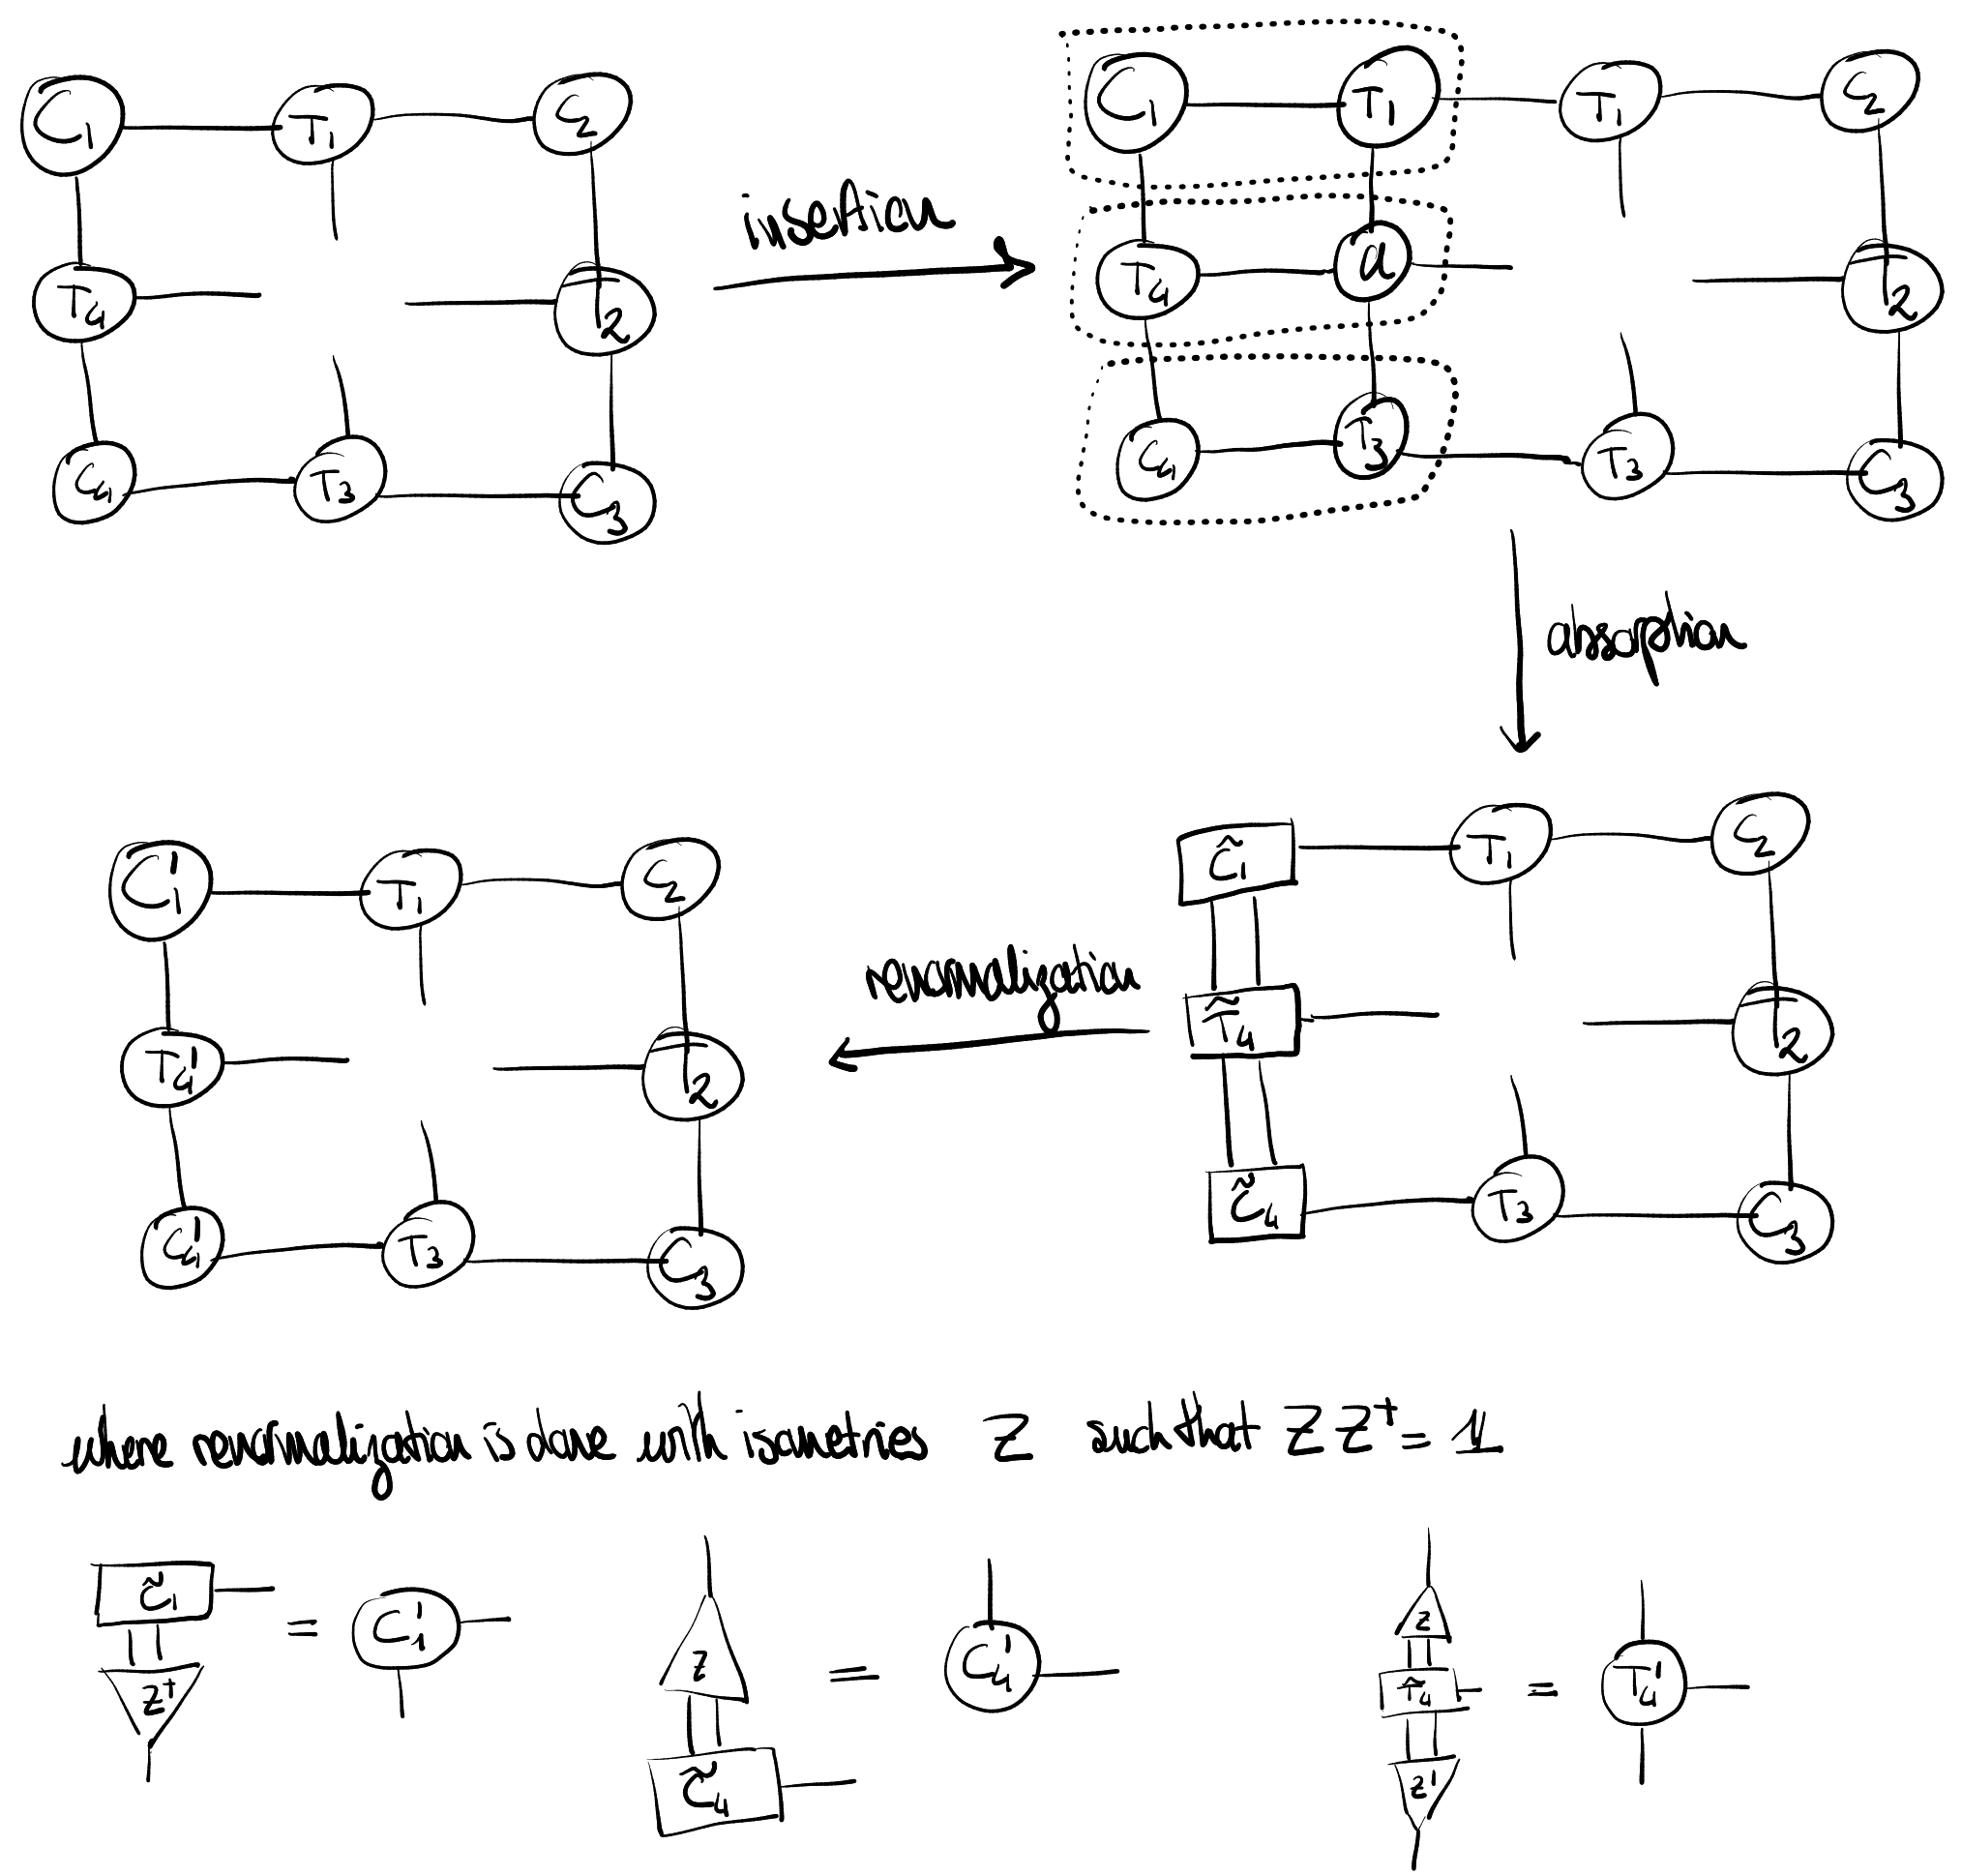
\includegraphics[scale=0.15]{graphs/ctmrgalgo.png}
            \caption{CTMRG algorithm.}
            \label{fig:ctmrgalgo}
        \end{figure}
    
    \section{Ground state research}
        
        Now that the structural ansatz of TN were established and that one knows how to approximate many-body state of a physical system. One is interested in finding the ground state of such systems. So will present two methods and we will focus on the second one which is widely used in a lot of fields in physics.
        
        First, the variational approach, that is based on the fact that the energy associated to the ground state is the lowest so that
        \begin{equation}
            E_0 < \frac{\bra{\Psi}H\ket{\Psi}}{\bra{\Psi}\ket{\Psi}}
        \end{equation}
        Thus minimizing the RHS of this inequality will give approximation of the ground state. In a TN formalism one could choose a family of state $\mc F$ --- MPS, PEPS... --- and minimize with respect to it. Only have one constraint which is the norm of the state to equal one. Thus introduce one Lagrange multiplier $\lambda$
        \begin{equation}
            \min_{\ket{\Psi} \in \mc F}(\bra{\Psi}\mc H\ket{\Psi} - \lambda \bra{\Psi}\ket{\Psi})
        \end{equation}
        If the state are defined as MPS state for example one should take every parameters of every tensor of the network as the variational parameters. Instead, fix every tensor but one and minimize with respect to it then move to another one and so on. In practice, perform that several times before reaching an acceptable approxiamtion of the ground state. So now fixing all the tensors but one gives
        \begin{equation}
            \min_{\ket{\Psi} \in F}(\bra{\Psi}H\ket{\Psi} - \lambda \bra{\Psi}\ket{\Psi}) = \min_A(\Vec{A}^{\dagger}H_{eff}\Vec{A} - \lambda\Vec{A}^{\dagger}N\Vec{A})
        \end{equation}
        where $\Vec{A}$ is the vectorly ordered tensor A, $\mc H_\text{eff}$ is an effective Hamiltonian and $\mc N$ a normalisation matrix. Usually $\mc H_\text{eff}$ and $N$ are respectively the TNs approximation of $\bra{\Psi}\mc H\ket{\Psi}$ and $\bra{\Psi}\ket{\Psi}$. Finally minimizing leads to the generalized eigenvalue problem
        \begin{equation}
            \mc H_\text{eff}\Vec{A} = \lambda \mc N\Vec{A}
        \end{equation}
        Note that for MPS with open boundary conditions, one just recovers the DMRG algorithm.

        A second method is the imaginary time evolution. The idea is taking a random state with non-zero overlap with the ground state and let it evolve with respect to an imaginary time such that
        \begin{equation}
            \ket{GS} = \lim_{\tau \rightarrow \infty}\frac{e^{-\tau \mc H}\ket{\psi}}{\sqrt{\bra{\psi}\ket{\psi}}}
        \end{equation}
        In order to prove this, take the Schrödinger equation
        \begin{equation}
            i\hbar\frac{\partial\psi(x,t)}{\partial t} = \mc H\psi(x,t)
        \end{equation}
        The global solution is given by
        \begin{equation}
            \psi(x,t) = \sum_n c_n(0)e^{-iE_nt/\hbar}\psi_n
        \end{equation}
        where $\psi_n$ are the eigenstates of the Hamiltonian, found by solving the eigenvalue problem. The time dependence is such that the eigenstates are oscillating in the representation of the evolving state one is considering. Now make the change of coordinate $t\rightarrow it = \tau$. The Schrödinger equation becomes
        \begin{equation}
            -\hbar\frac{\partial\psi(x,\tau)}{\partial \tau} = \mc H\psi(x,\tau)
        \end{equation}
        So that the general solution recasts as
        \begin{equation}
            \psi(x,t) = \sum_n c_n(0)e^{-E_n\tau/\hbar}\psi_n
        \end{equation}
        The interesting thing with that transformation is that one no longer has a superposition of oscillating eigenstate but an exponentially decaying superposition of those. So finally, if the random state chosen has a non-zero overlapping with the ground state, it belongs to the superposition and for a long imaginary time the dominating term would be $e^{-E_0\tau/\hbar}$. Hence end up with
        \begin{equation}
            \psi(x,\tau \gg 1) \simeq c_0(0)e^{E_0\tau/\hbar}\ket{\psi_0}
        \end{equation} 
        Re-normalising this state gives an approximation of the ground state.

    \section{Trotter-Susuki decomposition}

        Having the Imaginary time evolution method, one would like to apply the evolution operator on a MPS state one can take the case of a $1$D chain and consider only first neighbours interaction as
        \begin{equation}
            \hat{\mc H} = \sum_n \hat{h}_{n,n+1}
        \end{equation}
        One can perform a subdivision on the imaginary time $\tau$ so that the evolution factor becomes
        \begin{equation}
            e^{-\tau \mc H} = \left(e^{-\delta\tau \mc H}\right)^m
        \end{equation}
        Now in order to expand this exponentiation of operator, need the Trotter formula
        \begin{equation}
            e^{A+B} = \lim_{n\rightarrow\infty}\left(e^{\frac{A}{n}\frac{B}{n}}\right)^n
        \end{equation}
        One will need a generalisation of this expression since there are more than two non-commuting operators in the exponential. This generalisation has been proposed by Suzuki. First propose a systematic approximate for the exponential function based on its two equivalent formulations. 
        \begin{equation}
            e^x = \lim_{n\rightarrow\infty}\left(1+\frac{x}{n}\right)^n
        \end{equation}
        and
        \begin{equation}
            e^x = \lim_{m\rightarrow\infty}\sum^m_k\frac{x^k}{k!}
        \end{equation}
        Thus define the double index sequence
        \begin{equation}
            e_{n,m}(x) = \left(\sum^m_k\frac{\left(\frac{x}{n}\right)^k}{k!}\right)^n
        \end{equation}
        This sequence converges for both $n$ and $m$ to the exponential of $x$ as one can find the relation
        \begin{equation}
            \abs{e^x - e_{n,m}(x)} \leq \frac{\abs{x}^{m+1}}{n^m(m+1)!}e^{\abs{x}}
        \end{equation}
        For any operator in a Banach algebra this identity holds. Now for a collection of operator ${A_j}$ in a Banach algebra, get the following inequality which is the main result of Suzuki that is interesting here
        \begin{equation}
            \norm{\exp{\sum^p_j A_j} - f_n({A_j})} \leq \frac{2}{n}\left(\sum^p_j \norm{A_j}\right)^2 \exp{\frac{n+2}{n}\sum^p_j \norm{A_j}}
        \end{equation}
        where $p$ is an integer and $f_n({A_j}) = [e^{A_1/n}e^{A_2/n}e^{A_3/n}...e^{A_p/n}]^n$. Thus one sees that for $p=2$ one retrieves the Trotter formula and now a well-defined generalisation of this result that can applies of the factor $e^{-\tau H}$. Finally the first order Trotter-Suzuki decomposition reads
        \begin{equation}
            e^{-\delta\tau \mc H} = \prod_n e^{-\delta\tau h_{n,n+1}} + O(\delta\tau^2)
        \end{equation}
        There are several ways to apply that imaginary time evolution on an MPS state and thanks to the Trotter-Suzuki decomposition it takes a quite straightforward from as is \autoref{fig:imaginaryevtn}.
        
        \begin{figure}[!h]
            \centering
            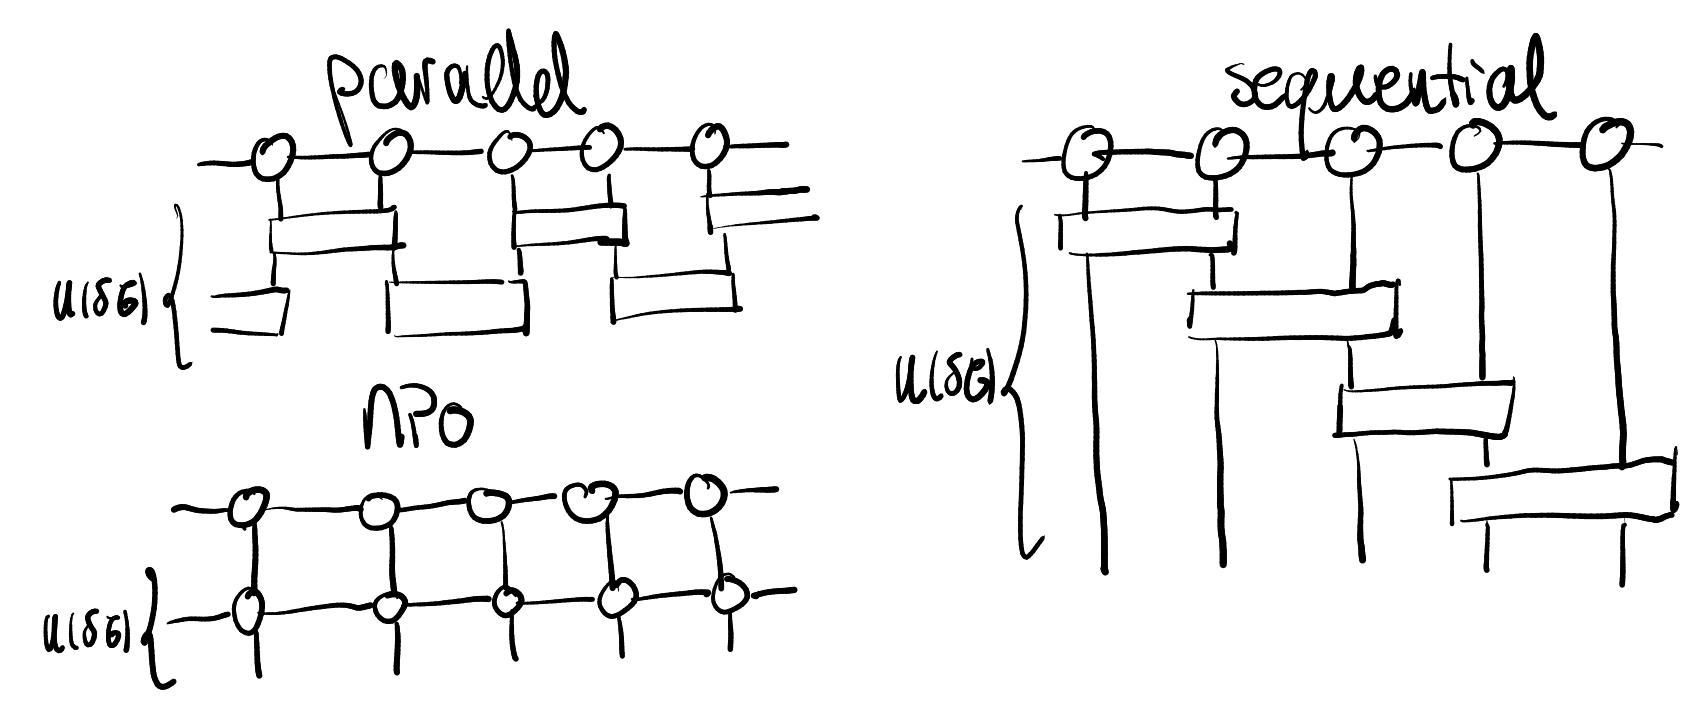
\includegraphics[scale=0.2]{graphs/imaginaryevtn.png}
            \caption{Application of the imaginary time evolution operator on an MPS state/}
            \label{fig:imaginaryevtn}
        \end{figure}

    \section{iTEBD in 1D}

        So far, we have only used MPS notation based on one set of matrices --- the $A$-matrices --- per site, but there also exists other useful notations, such as the one introduced by Vidal which takes the form
        \begin{equation}
            \ket{\psi}=\sum_{\sigma_1,\dots,\sigma_L}\Gamma^{\sigma_1}\lambda^{[1]}\Gamma^{\sigma_2}\lambda^{[2]}\dots\Gamma^{\sigma_{L-1}}\lambda^{[L-1]}\Gamma^{\sigma_L}\ket{\vec{\sigma}}
        \end{equation}
        where was introduced on each site $\ell$ a set of $d$ matrices $\Gamma^{\sigma_{\ell}}$ and on each bond $\ell$ one diagonal matrix $\lambda^{[\ell]}$. This is just another way of reshaping the wavefunction coefficients. These matrices are specified by the demand that for arbitrary $\ell$ ($1\leq \ell<L$) one can read off the Schmidt decomposition
        \begin{equation}
            \ket{\psi}=\sum_{a_{\ell}}^rs_{a_{\ell}}\ket{a_{\ell}}_\text{A}\ket{a_{\ell}}_\text{B}
        \end{equation}
        with $r$ the Schmidt rank and where the Schmidt coefficients are the diagonal elements of $\lambda^{[\ell]}$, namely $s_{a_{\ell}}=\lambda^{[\ell]}_{a_{\ell} a_{\ell}}$ and the states on A and B are given as
        \begin{align*}
            \ket{a_{\ell}}_\text{A}&=\sum_{\sigma_1,\dots,\sigma_{\ell}}\left(\Gamma^{\sigma_1}\lambda^{[1]}\Gamma^{\sigma_2}\dots\lambda^{[\ell-1]}\Gamma^{\sigma_{\ell}}\right)_{a_{\ell}}\ket{\sigma_1,\dots,\sigma_{\ell}}\,,\\
            \ket{a_{\ell}}_\text{B}&=\sum_{\sigma_{\ell+1},\dots,\sigma_L}\left(\Gamma^{\sigma_{\ell+1}}\lambda^{[\ell+1]}\Gamma^{\sigma_{\ell+2}}\dots\lambda^{[L-1]}\Gamma^{\sigma_{L}}\right)_{a_{\ell}}\ket{\sigma_{\ell+1},\dots,\sigma_{L}}\,,
        \end{align*}
        where the states on A and B are orthonormal respectively, similarly to the constructions of $A$ and $B$ matrices. Graphically, the new notation can be represented as in \autoref{fig:vidalnotation}.

        \begin{figure}[!h]
            \centering
            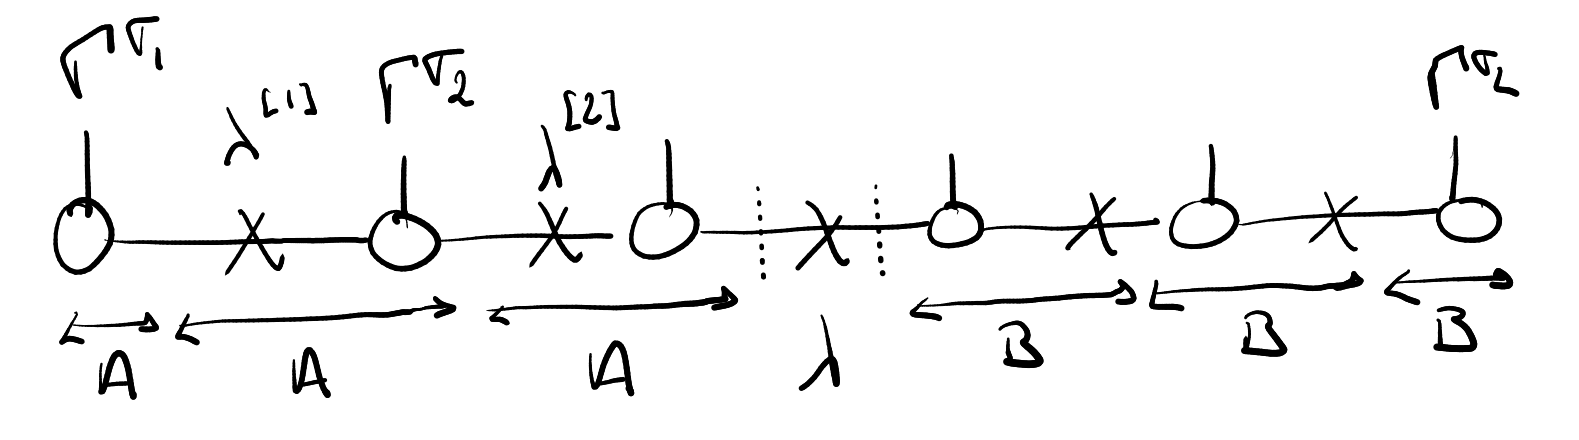
\includegraphics[scale=0.2]{graphs/vidalnotation.png}
            \caption{Pictural representation of the $\Gamma-\lambda$ notation.}
            \label{fig:vidalnotation}
        \end{figure}

        The crucial difference to the decomposition into $A$-matrices is that each $A$ is decomposed, using the knowledge of $\lambda^{[\ell-1]}$ obtained in the previous step, into
        \begin{equation}
            A_{a_{\ell-1},a_{\ell}}^{\sigma_{\ell}}=\lambda_{a_{\ell-1},a_{\ell-1}}^{[\ell-1]}\Gamma_{a_{\ell-1},a_{\ell}}^{\sigma_{\ell}}
        \end{equation}
        Similarly, decompose from the right using the right-normalization of $B$-matrices, the same state is obtained with a grouping
        \begin{equation}
            B_{a_{\ell-1},a_{\ell}}^{\sigma_{\ell}}=\Gamma_{a_{\ell-1},a_{\ell}}^{\sigma_{\ell}}\lambda_{a_{\ell},a_{\ell}}^{[\ell]}
        \end{equation}

        The TEBD algorithm, which stands for Time-Evolving Block Decimation, is a numerical scheme to simulate the evolution of a 1D finite lattice. But bulk properties of matter are best studied in an infinite system, where they are not contaminated by finite-size corrections or boundary effects. However, for most algorithms the cost of a simulation grows with the system size, and the thermodynamic limit can only be reached by extrapolating results for increasingly large systems. Present here the infinite TEBD, conveniently abridged iTEBD, a noticeably simple and fast algorithm to simulate infinite systems directly, without even resorting to extrapolations.

        As presented before, the Trotter-Suzuki decomposition allows to expand the evolution operator as a sequence of small two-site gates
        \begin{equation}
            \mathcal{U}_{\ell,\ell+1}\equiv\exp{-i h_{\ell,\ell+1}\delta t},\quad\delta t \ll 1
        \end{equation}
        In the TEBD algorithm, arrange the evolution operator into two gates $\mathcal{U}^\text{AB}$ and $\mathcal{U}^\text{BA}$
        \begin{equation}
            \mathcal{U}^\text{AB}\equiv\bigotimes_{\ell\in\mathbb{Z}}\mathcal{U}_{2\ell,2\ell+1}\,,\quad\mathcal{U}^\text{BA}\equiv\bigotimes_{\ell\in\mathbb{Z}}\mathcal{U}_{2\ell-1,2\ell}\,.
        \end{equation}
        The wavefunction $\ket{\psi}$ is shift invariant, therefore it can be represented with an MPS where $\Gamma^{\sigma_\ell}$ and $\lambda^{[\ell]}$ are actually independent of $\ell$. However, one will partially break this translational symmetry in order to simulate the action of the two previous gates on $\ket{\psi}$. To this end, choose an MPS of the form
        \begin{gather}
            \Gamma^{\sigma_{2\ell}}=\Gamma^\text{A}\,,\quad\lambda^{[2\ell]}=\lambda^\text{A}\\
            \Gamma^{\sigma_{2\ell+1}}=\Gamma^\text{B}\,,\quad\lambda^{[2\ell+1]}=\lambda^\text{B}\,,\quad\ell\in\mathbb{Z}
        \end{gather}
        The TEBD considers a finite $L$ sites case, where the simulation of the time evolution is achieved by updating the MPS with repeated applications of gates $\mathcal{U}^\text{AB}$ and $\mathcal{U}^\text{BA}$ on $\ket{\psi}$. For the infinite TEBD, that is for $L=\infty$, the action of the gates preserves the invariance of the evolved state under shifts of two sites, as shown in \autoref{fig:invarianceitebd}. In the first part, one has drawn a tensor network representation containing both an MPS for $\ket{\psi}$ and two-site gates $\mathcal{U}$ acting on each pair of sites $\{2\ell, 2\ell+1\}$. On the second part, drawn the new MPS obtained, which is $\mathcal{U}^\text{AB}\ket{\psi}$. Notice that both structures are invariant under shifts by two lattice sites and are completely specified by a handful of tensors, despite the fact that they represent a state of an infinite 1D lattice.

        \begin{figure}[!h]
            \centering
            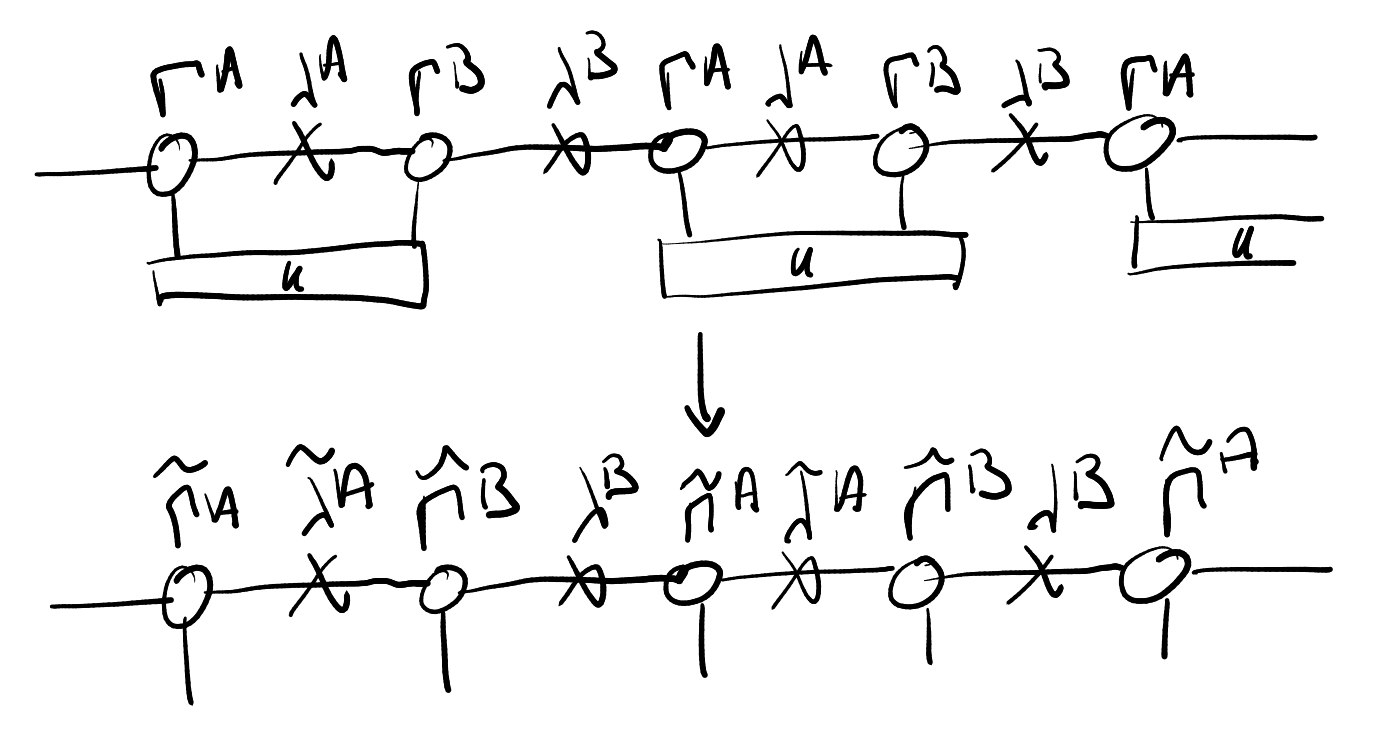
\includegraphics[scale=0.2]{graphs/invarianceitebd.png}
            \caption{Shift-invariance of the structure.}
            \label{fig:invarianceitebd}
        \end{figure}

        Therefore only tensors $\Gamma^\text{A}$, $\Gamma^\text{B}$, $\lambda^\text{A}$, and $\lambda^\text{B}$ need to be updated, which can be achieved through simple matrix manipulations shown in \autoref{fig:MPSupdate}. In order to update the MPS after gate $\mathcal{U}$ has been applied, first contract the tensor network into a single tensor $\Theta_{\alpha ij\gamma}$. Then perform an SVD of $\Theta$ according to the index bipartition $(\alpha i):(j\gamma)$, namely
        \begin{equation}
            \Theta=\sum_{\beta}X_{(\alpha i),\beta}\Tilde{\lambda}_\beta^\text{A}Y_{\beta(j\gamma)}\,.
        \end{equation}
        We can introduce $\lambda^\text{B}$ back into the network using the inverse matrix $(\lambda^\text{B})^{-1}$ and we can form tensors $\Tilde{\Gamma}^\text{A}$ and $\Tilde{\Gamma}^\text{B}$ by attaching $X$ and $Y$ to it. 
        \begin{figure}[h!]
            \centering
            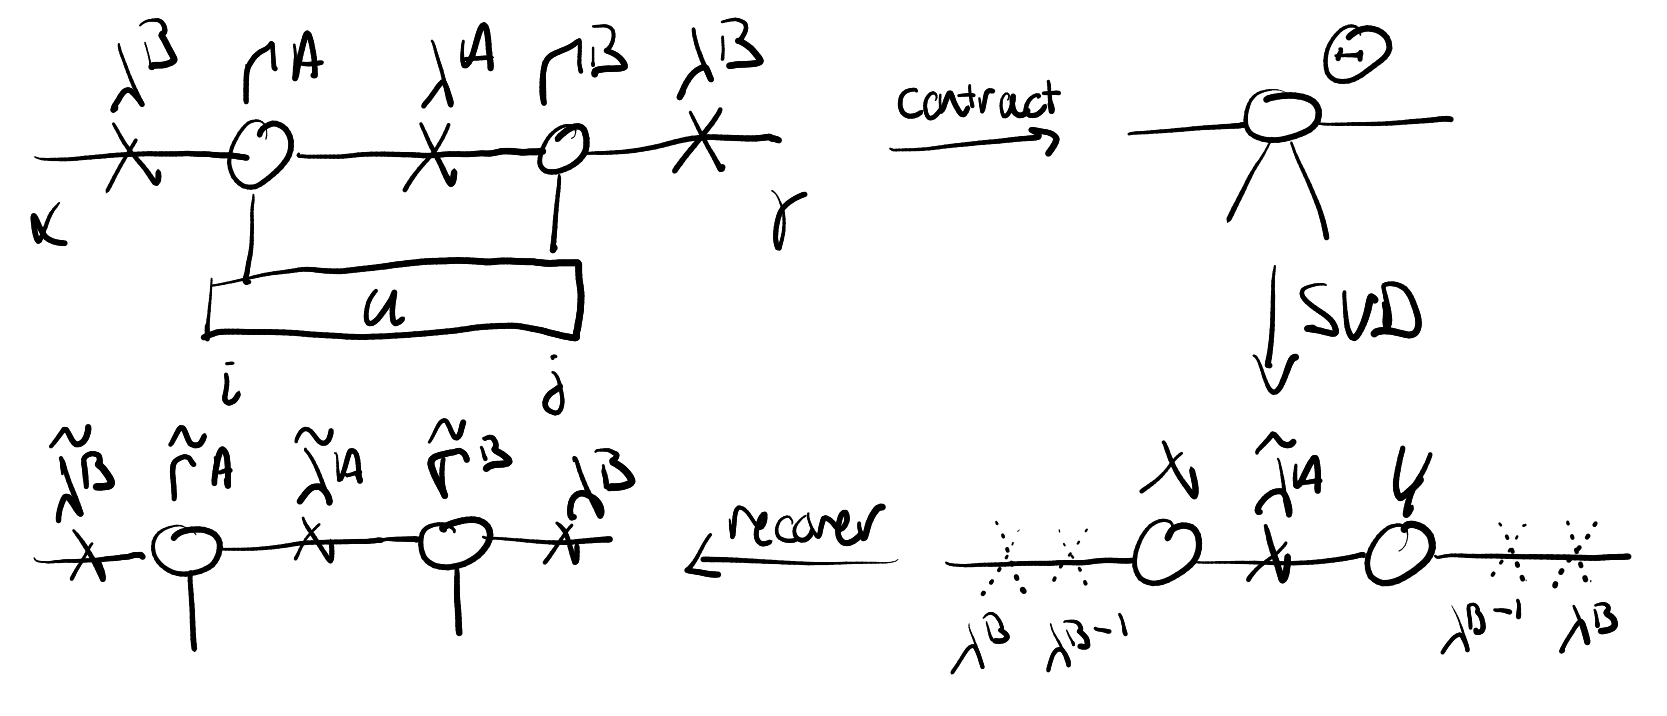
\includegraphics[scale=0.2]{graphs/MPSupdate.png}
            \caption{MPS update in iTEBD.}
            \label{fig:MPSupdate}
        \end{figure}

        For $L$ sites, the TEBD algorithm requires $\mathcal{O}(Ldr^2)$ space to store an MPS and $\mathcal{O}(Ld^3r^3)$ time to simulate a small evolution $\exp{-i H\delta t}$. For $L$ sites, the iTEBD requires computational space and time that scale just as $\mathcal{O}(d^2r^2)$ and $\mathcal{O}(d^3r^3)$. The key to such a drastic cost reduction by a factor $L$ is that, in contrast to other approaches, here use an MPS based on the Schmidt decomposition, allowing for a parallelized and local update of tensors $\Gamma$ and $\lambda$.

        Finally, evolution in imaginary time can also be simulated with iTEBD by simply replacing the two-site unitary gates $\exp{-i h\delta t}$ with non-unitary gates $\exp{-h\delta\tau}$, $\delta\tau\ll 1$.\\
        Note that nonunitary gates destroy the Schmidt decomposition. A parallelized and local update of tensors should no longer be possible. For small $\delta\tau,$ however, gate $\exp{-h\delta\tau}$ is close to the identity, and proceeding with a local update introduces only small errors that vanish as $\delta\tau\longrightarrow 0$. An accurate MPS for the ground state $\ket{\text{GS}}$ is then achieved by simulating imaginary time evolution with decreasingly small values of $\delta\tau$.//

        There are simple extensions of the algorithm, which include, only to name a few
        \begin{itemize}
            \item Interactions $h$ with longer range. Here only considered next-nearest neighbor interactions.
            \item Interactions involving more than just two sites \emph{eg} $h_{\ell,\ell+1,\ell+2}$.
            \item Time-dependent hamiltonians.
            \item Systems invariant under shifts by $m$ sites, with $m>1$, \emph{ie}. a larger unit cell.
        \end{itemize}

    \section{Evolution of iPEPS}

        The goal is to find the ground state of an Hamiltonian with only the nearest-neighbor interactions in a $2$D lattice. To do so, use iPEPS to find an approximation. The procedure consists in projecting-out the ground state via the imaginary time evolution as
        \be \ket{\psi_0} = \lim_{\tau\to\infty} \frac{e^{-\tau\mc H} \ket \psi}{\norm{e^{-\tau\mc H} \ket \psi}} \ee
        The goal is to apply the gate successively, exactly as for MPS in the iTEBD. But for MPS the truncation can be done in an optimal way casting them in canonical form and doing SVD. For iPEPS, no canonical form exist. It can be viewed by the iPEPS having loops in general, then the environment is not separable. Hence, use approximation in the truncation via simple or full update.

    \section{Simple update}
        
        Consider as an example that will guide the description of the procedure, the spin-$\frac 1 2$ Heisenberg model on the honeycomb lattice. The Hamiltonian can be written 
        \be \begin{split} \mc H &= \sum_{\ev{ij}} \mc H_{ij} \\ &= \sum_{\ev{ij}} J \vb* S_i\cdot \vb* S_j - \frac{h}{2}\left[(-1)^i S_i^z + (-1)^j S_j^z \right] \end{split} \ee
        Schematically, the TN state is as in \autoref{fig:hcbtnsimple}, having attached diagonal matrices $\lambda_\alpha$, $\alpha=x,y,z$ to the bonds, that will be used to take into account an effective environment through them.

        \begin{figure}[h!]
            \centering
            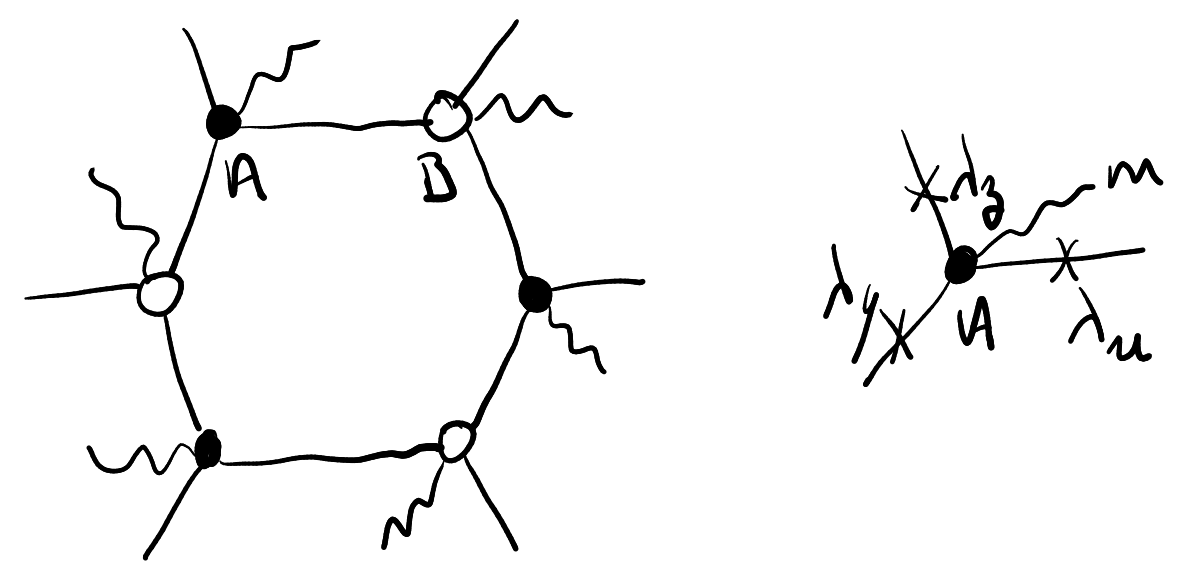
\includegraphics[scale=0.2]{graphs/hcbtnsimple.png}
            \caption{Spin-$\frac 1 2$ Heisenberg model on the honeycomb lattice as a tensor network.}
            \label{fig:hcbtnsimple}
        \end{figure}

        The system considered for the update is of the form given in \autoref{fig:syshcbtnsimple}. It is important to note that the bond indices $\alpha_i$ can take $D$ values.

        \begin{figure}[h!]
            \centering
            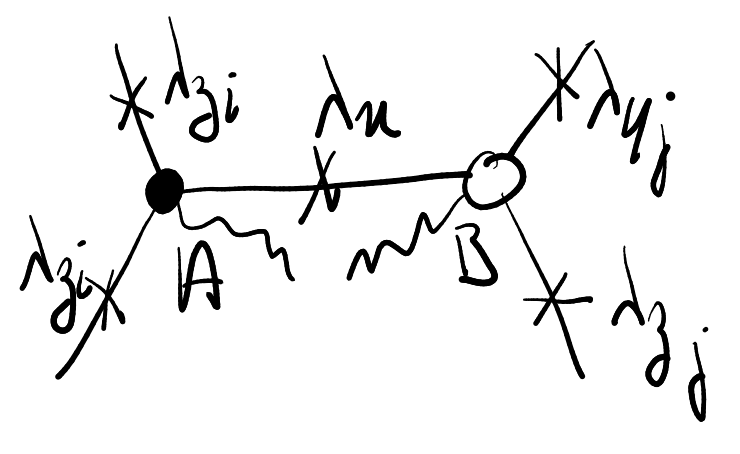
\includegraphics[scale=0.2]{graphs/syshcbtnsimple.png}
            \caption{System considered for the simple update.}
            \label{fig:syshcbtnsimple}
        \end{figure}

        Now, assume the state
        \be \ket \psi = \tr \prod_{i\in b,j\in w} \lambda_{x_i}\lambda_{y_i} \lambda_{z_i} A_{x_i y_i z_i}^{m_i} B_{x_j y_j z_j}^{m_j} \ket{m_i,m_j} \ee
        with the trace the sum over all spin configurations and all bonds indices. Divide the Hamiltonian
        \be \mc H = \sum_{\alpha=x,y,z} \mc H_\alpha \qq{with} \mc H_\alpha = \sum_{i\in b} \mc H_{i,i+\alpha} \ee
        Apply the Trotter-Susuki formula to split the evolution operator as
        \be e^{-\tau\mc H} = e^{-\tau\mc H_x}e^{-\tau\mc H_y}e^{-\tau\mc H_z} + \mc O(\tau^2) \ee
        and noticing by commutation
        \be e^{-\tau\mc H_\alpha} = \prod_{i\in b} \underbrace{e^{-\tau\mc H_{i,i+\alpha}}}_\text{gate} \ee
        To represent the simple update with diagrams, follow \autoref{fig:simpleupdatehcbtn}, where only the bond $x$ has been considered.

        \begin{figure}[h!]
            \centering
            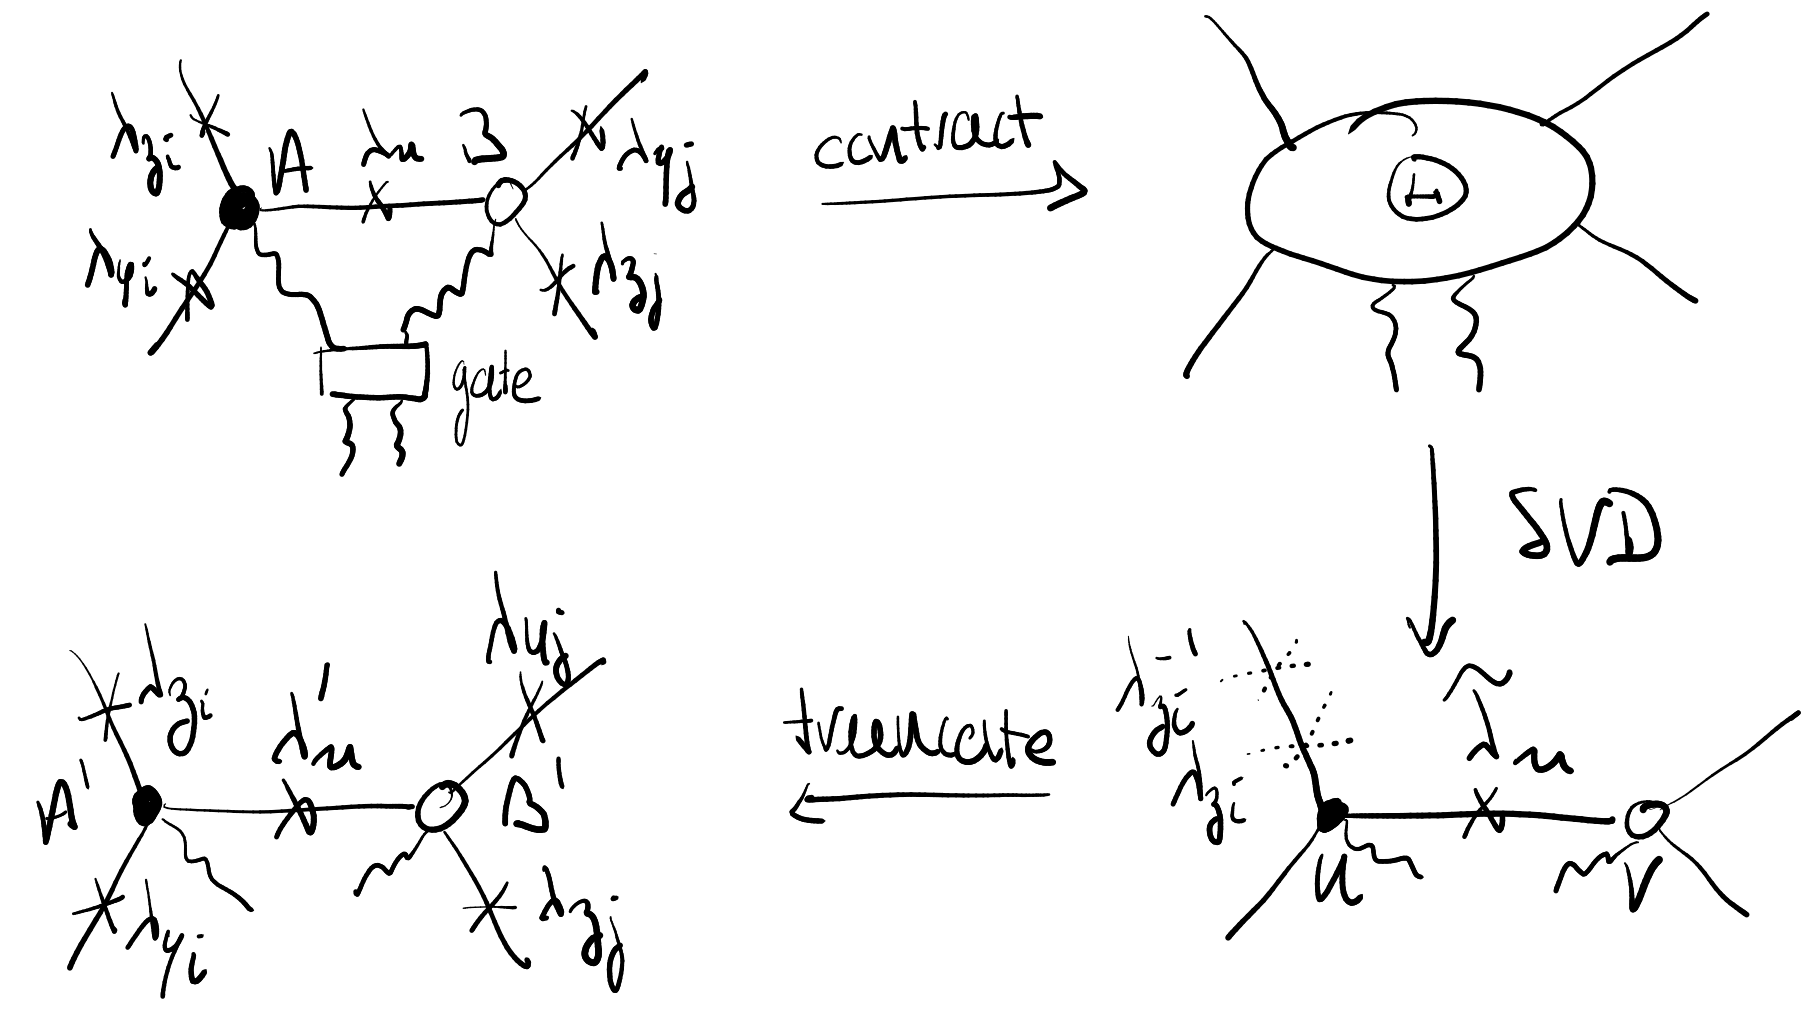
\includegraphics[scale=0.2]{graphs/simpleupdatehcbtn.png}
            \caption{Procedure of the simple update on the honeycomb lattice, only for the bond $x$ for simplicity.}
            \label{fig:simpleupdatehcbtn}
        \end{figure}

        Then, apply the same procedure for on the $y$- and $z$-bonds, being careful to the fact that the $\lambda$ matrices are only changed on the bond considered, keeping all the others unchanged, as mean-field. 

        With equations, one reads
        \be \begin{split} e^{-\tau\mc H_x} \ket \psi = \tr &\prod_{i\in b,j=i+x} \sum_{m_i',m_j'} \mel{m_i',m_j'}{\overbrace{e^{-\tau\mc H_{ij}}}^\text{gate}}{m_i,m_j} \\ &\cdot \lambda_{x_i}\lambda_{y_i} \lambda_{z_i} A_{x_i y_i z_i}^{m_i} B_{x_j y_j z_j}^{m_j} \ket{m_i',m_j'} \end{split} \ee
        The contraction gives a $D^2 d \times D^2 d$ matrix, with $d=2$ here as the dimension of the basis of a single-state Hilbert space,
        \be \begin{split} \Theta_{y_iz_im_i',y_jz_jm_j'} = &\sum_{m_i,m_j} \sum_x \mel{m_i',m_j'}{e^{-\tau\mc H_{ij}}}{m_i,m_j} \\ &\cdot \lambda_{y_i} \lambda_{z_i} A_{x y_i z_i}^{m_i} \lambda_x B_{x y_j z_j}^{m_j} \lambda_{y_j} \lambda_{z_j} \\ &\stackrel{\text{SVD}}{=} \sum_x U_{y_iz_im_i,x} \tilde \lambda_x V^\dagger{x,y_jz_jm_j} \end{split} \ee
        Then truncate the bond $ \tilde \lambda_x$ of dimension $D^2d$ back to $\lambda'_x$ of dimension $D$ and update
        \be \begin{split} A_{x y_i z_i}^{\prime m_i} &= \lambda^{-1}_{y_i} \lambda^{-1}_{z_i} U_{y_iz_im_i,x} \\ B_{x y_j z_j}^{\prime m_j} &= \lambda^{-1}_{y_j}\lambda^{-1}_{y_j} V_{y_jz_jm_j,x} \end{split} \ee

    \section{Full update}

        \begin{figure}[h!]
            \centering
            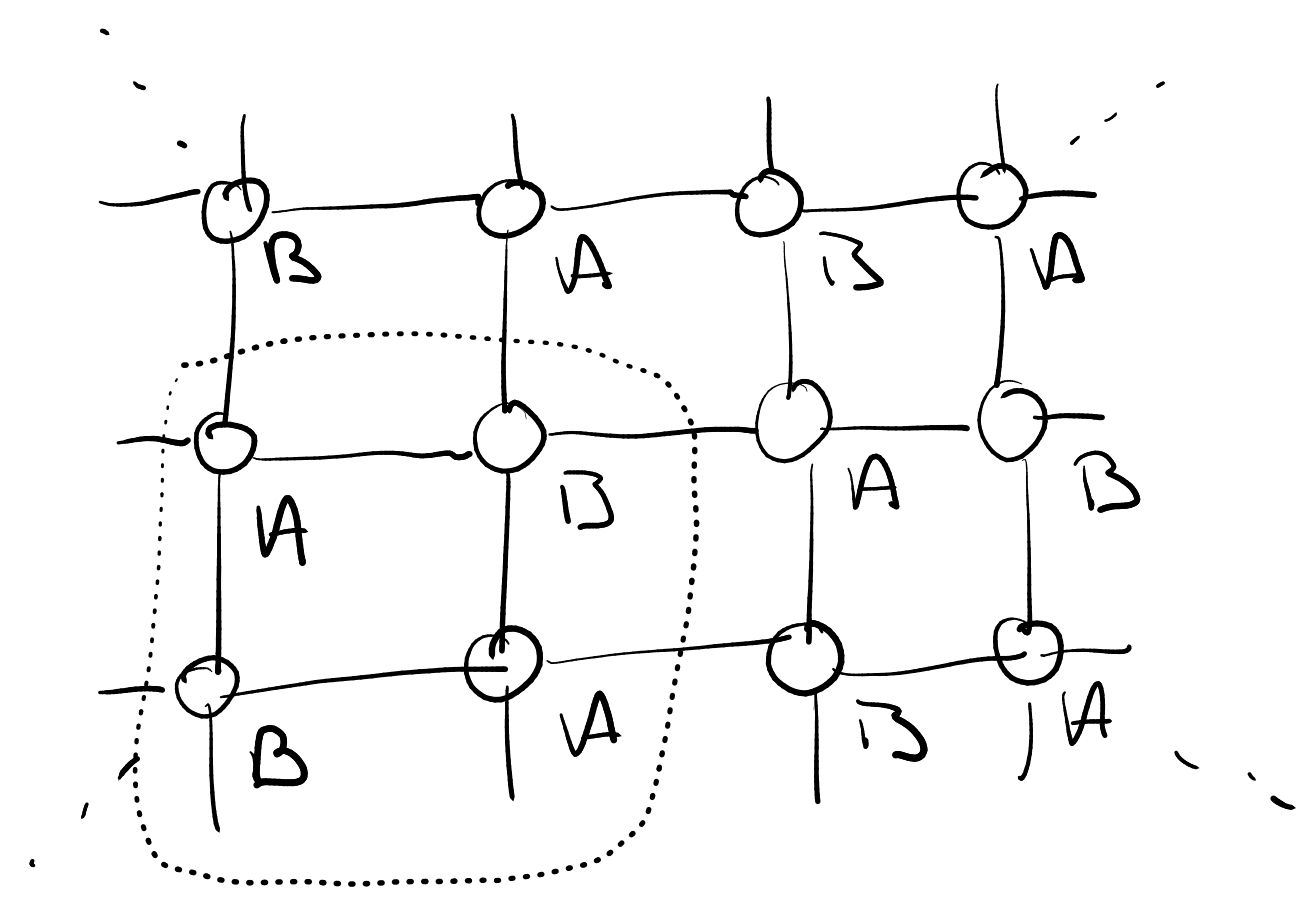
\includegraphics[scale=0.2]{graphs/fulltnlattice.png}
            \caption{Lattice considered for the full update procedure here.}
            \label{fig:fulltnlattice}
        \end{figure}

        To consider the full update, focus on one link with tensors $A$ and $B$ on \autoref{fig:fulltnlattice}. The iPEPS and its evolution is as
        \be \ket{\psi_{AB}} \xrightarrow{\text{apply gate}} \ket{\psi_{A'B'}} \xrightarrow{\text{truncate to }D} \ket{\psi_{\tilde A \tilde B}} \ee
        where only $A,B$ are changed, all the rest is fixed. The truncation is necessary to avoid the exponential increase of the bond dimension. A good way to perform this approximation is to find $\tilde A, \tilde B$ such that
        \be d(\tilde A, \tilde B) = \norm{\ket{\psi_{A'B'}} - \ket{\psi_{\tilde A \tilde B}}}^2 \ee
        is minimized. To solve this problem, one needs to
        \begin{enumerate}[label=${[\arabic*]}$]
            \item calculate the effective environment
            \item update the system
        \end{enumerate}
        For $[1]$, there are various approaches but focus on CTM methods.\\
        For $[2]$, the process is as follows
        \begin{itemize}
            \item fix $\tilde B$ to rewrite
            \be d(\tilde A, \tilde A^\dagger) = \tilde A^\dagger R \tilde A - \tilde A^\dagger S - S^\dagger \tilde A + T \ee
            with $ \tilde A$ having bond dimension $D$. The tensors $R$, $S$ and $T$ are given in \autoref{fig:fulltnrst}.

            \begin{figure}[h!]
                \centering
                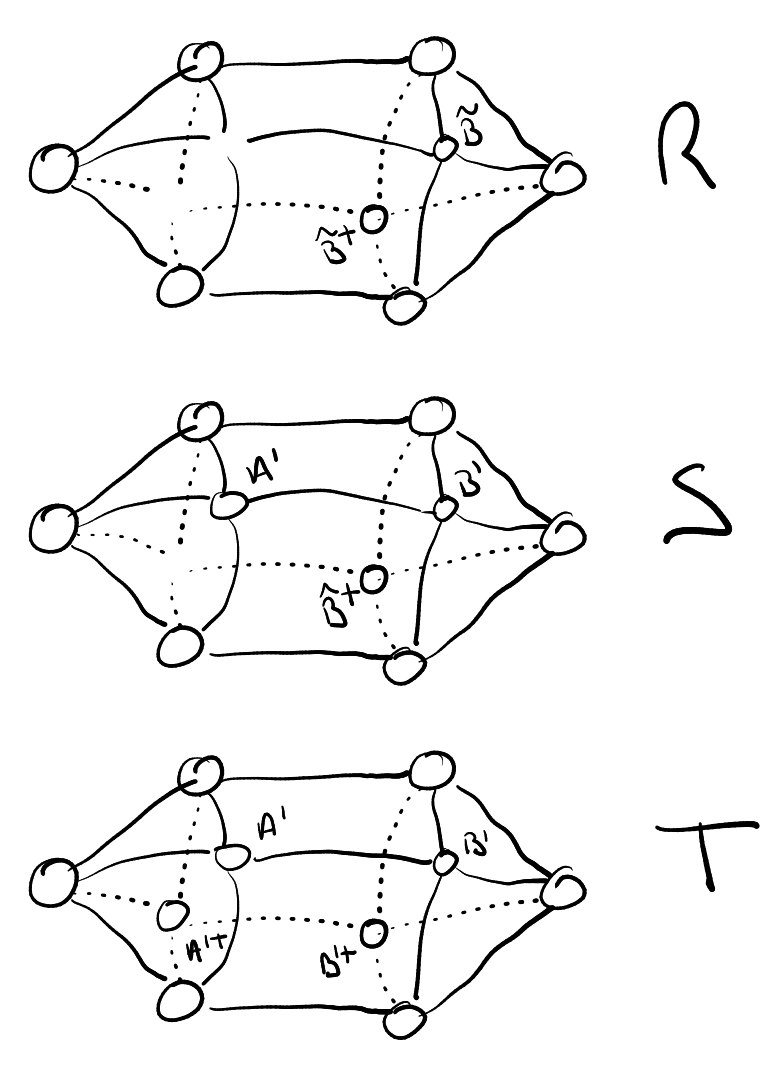
\includegraphics[scale=0.25]{graphs/fulltnrst.png}
                \caption{Tensors involved in the computation of the effective environment in the full update.}
                \label{fig:fulltnrst}
            \end{figure}

            \item find $\min_{\tilde A^\dagger} d(\tilde A,\tilde A^\dagger)$ thus 
            \be \pdv{d(\tilde A,\tilde A^\dagger)}{\tilde A^\dagger} = 0 \implies \tilde A = R^{-1} S \ee
            \item fix $\tilde A$ and do the same for $\tilde B$
            \item replace $\tilde A,\tilde B$ over the entire lattice to represent the effect of all the corresponding gates
            \item repeat for the other $3$ bonds
        \end{itemize}

        There are number of ways to make it faster
        \begin{itemize}
            \item optimize the computation of $R^{-1}$
            \item (applicable to simple update) do QR/LQ or SVD on $A$ and $B$ and apply the gate on those that have less components
            \item fast full update, where the effective environment and the tensors are updated simultaneously
            \item gauge fixing, which improves stability too
            \item ...
        \end{itemize}
